\section{Details of the Code}
\label{Code}
\subsection{Directory structure}
The directory structure is as shown in Fig.\ \ref{fdirs}, with the
ability to run the ocean alone or coupled to atmospheric and/or
wave models. If running just the ocean, the model can be run forward
in time (the nonlinear model) or as an adjoint, tangent linear, or
representer model for data assimilation purposes. This document
describes the uncoupled forward model only, specifically the version
used for the Northeast Pacific domain containing sea ice and other
changes from the main trunk code. Details are subject to change
without notice - check your own source code for specific details as
they apply to you.

The directories shown here are:
\begin{klist}
  \kitem{Apps} This directory contains a subdirectory for each of my
  personal applications. The subdirectory contains files used by that
  application: the ROMS header file for setting cpp definitions, the
  analytic formulations for fields computed in the model rather than
  read from files (bottom heat flux of zero, for instance), and ASCII
  input files read by ROMS on startup to set things such as forcing file
  names and model timestep. Some of these applications are:
\begin{klist}
  \kitem{Bering} This is a 4 km grid of the Bering Sea, aligned with
  the Northeast Pacific grid but at three times the resolution.
  \kitem{Bering\_10k} This is a 10 km grid of the Bering Sea, a
  subset of the Northeast Pacific domain, with the same extent as
  the 4 km grid above.
  \kitem{CGOA} This is a 3 km grid of the Gulf of Alaska. It is a
  subset of the Northeast Pacific grid, but at four times the
  resolution.
  \kitem{Circle} This is a circular domain wave propagation problem
  with an analytic solution used as a test problem (\cite{Lamb32}).
  \kitem{NEP} This is the Northeast Pacific domain covering the
  waters off the west coast of the US, from California to the Bering
  Sea. It is a rectangular domain at about 11 km resolution when
  viewed in a conformal conic projection with standard latitudes of
  40 and 60 N.
\end{klist}
  Paul Budgell's applications are also here. The application-specific
  files included in the main trunk ROMS are elsewhere.
  \kitem{Atmosphere} This directory is under development, not
  currently supported.
  \kitem{Compilers} This contains makefile fragments as described in
  \S\ref{Mult_dir_make}.
  \kitem{Data} Directories under here contain example forcing, grid,
  and initial condition NetCDF files. There is also a directory
  containing the headers of these files in the format produced by
  \code{ncdump} (CDL).
  \kitem{Lib} The ARPACK and MCT libraries are needed by the data
  assimilation codes and by the coupled models, respectively.
  \kitem{makefile} This is the standard ROMS makefile as described
  in \S\ref{Gmake}.
  \kitem{Master} The ROMS main program is here, in various forms for
  the forward model, coupled models and others. See \S\ref{Master}.

\begin{figure}[t]
\thinlines
\begin{center}
\setlength{\unitlength}{3947sp}%
%
\begin{picture}(5505,5286)(1486,-7276)
\put(6976,-5461){\makebox(0,0)[lb]{{{{\color[rgb]{0,0,0}Sediment/}%
}}}}
\put(3376,-3061){\makebox(0,0)[lb]{{{{\color[rgb]{0,0,0}Circle/}%
}}}}
\put(3376,-2761){\makebox(0,0)[lb]{{{{\color[rgb]{0,0,0}CGOA/}%
}}}}
\put(3376,-2461){\makebox(0,0)[lb]{{{{\color[rgb]{0,0,0}Bering\_10k/}%
}}}}
\put(3376,-2161){\makebox(0,0)[lb]{{{{\color[rgb]{0,0,0}Bering/}%
}}}}
\put(4876,-2761){\makebox(0,0)[lb]{{{{\color[rgb]{0,0,0}Adjoint/}%
}}}}
\put(4876,-3061){\makebox(0,0)[lb]{{{{\color[rgb]{0,0,0}Bin/}%
}}}}
\put(4876,-3361){\makebox(0,0)[lb]{{{{\color[rgb]{0,0,0}Drivers/}%
}}}}
\put(4876,-3661){\makebox(0,0)[lb]{{{{\color[rgb]{0,0,0}External/}%
}}}}
\put(4876,-3961){\makebox(0,0)[lb]{{{{\color[rgb]{0,0,0}Functionals/}%
}}}}
\put(4876,-4261){\makebox(0,0)[lb]{{{{\color[rgb]{0,0,0}Include/}%
}}}}
\put(4876,-4561){\makebox(0,0)[lb]{{{{\color[rgb]{0,0,0}License\_ROMS.txt}%
}}}}
\put(4876,-4861){\makebox(0,0)[lb]{{{{\color[rgb]{0,0,0}Modules/}%
}}}}
\put(4876,-5161){\makebox(0,0)[lb]{{{{\color[rgb]{0,0,0}Nonlinear/}%
}}}}
\put(4876,-5461){\makebox(0,0)[lb]{{{{\color[rgb]{0,0,0}Obsolete/}%
}}}}
\put(4876,-5761){\makebox(0,0)[lb]{{{{\color[rgb]{0,0,0}Programs/}%
}}}}
\put(4876,-6061){\makebox(0,0)[lb]{{{{\color[rgb]{0,0,0}Representer/}%
}}}}
\put(4876,-6361){\makebox(0,0)[lb]{{{{\color[rgb]{0,0,0}SeaIce/}%
}}}}
\put(4876,-6661){\makebox(0,0)[lb]{{{{\color[rgb]{0,0,0}Tangent/}%
}}}}
\put(4876,-6961){\makebox(0,0)[lb]{{{{\color[rgb]{0,0,0}Utility/}%
}}}}
\put(4876,-7261){\makebox(0,0)[lb]{{{{\color[rgb]{0,0,0}Version}%
}}}}
\thinlines
{\color[rgb]{0,0,0}\put(2251,-4486){\line( 1, 0){2550}}
}%
{\color[rgb]{0,0,0}\put(2101,-2386){\line( 1, 0){900}}
}%
{\color[rgb]{0,0,0}\put(4501,-4561){\line( 0, 1){1875}}
\put(4501,-2686){\line( 1, 0){300}}
}%
{\color[rgb]{0,0,0}\put(4501,-2986){\line( 1, 0){300}}
}%
{\color[rgb]{0,0,0}\put(4501,-3286){\line( 1, 0){300}}
}%
{\color[rgb]{0,0,0}\put(4501,-3586){\line( 1, 0){300}}
}%
{\color[rgb]{0,0,0}\put(4501,-4486){\line( 0,-1){2700}}
\put(4501,-7186){\line( 1, 0){300}}
}%
{\color[rgb]{0,0,0}\put(4501,-3886){\line( 1, 0){300}}
}%
{\color[rgb]{0,0,0}\put(4501,-4186){\line( 1, 0){300}}
}%
{\color[rgb]{0,0,0}\put(4801,-4486){\line( 0, 1){  0}}
}%
{\color[rgb]{0,0,0}\put(4501,-4786){\line( 1, 0){300}}
}%
{\color[rgb]{0,0,0}\put(4501,-5086){\line( 1, 0){300}}
}%
{\color[rgb]{0,0,0}\put(4501,-5386){\line( 1, 0){300}}
}%
{\color[rgb]{0,0,0}\put(4501,-5686){\line( 1, 0){300}}
}%
{\color[rgb]{0,0,0}\put(4501,-5986){\line( 1, 0){300}}
}%
{\color[rgb]{0,0,0}\put(4501,-6286){\line( 1, 0){300}}
}%
{\color[rgb]{0,0,0}\put(4501,-6586){\line( 1, 0){300}}
}%
{\color[rgb]{0,0,0}\put(4501,-6886){\line( 1, 0){300}}
}%
{\color[rgb]{0,0,0}\put(3001,-2386){\line( 1, 0){300}}
}%
{\color[rgb]{0,0,0}\put(3001,-2686){\line( 1, 0){300}}
}%
{\color[rgb]{0,0,0}\put(3001,-2086){\line( 0,-1){1200}}
\put(3001,-3286){\line( 1, 0){300}}
}%
{\color[rgb]{0,0,0}\put(3001,-2986){\line( 1, 0){300}}
}%
{\color[rgb]{0,0,0}\put(3001,-2086){\line( 1, 0){300}}
}%
{\color[rgb]{0,0,0}\put(5926,-5086){\line( 1, 0){975}}
\put(6901,-5086){\line(-1, 0){300}}
\put(6601,-5086){\line( 0,-1){300}}
\put(6601,-5386){\line( 1, 0){300}}
}%
\put(1501,-2761){\makebox(0,0)[lb]{{{{\color[rgb]{0,0,0}Atmosphere/}%
}}}}
\put(1501,-3061){\makebox(0,0)[lb]{{{{\color[rgb]{0,0,0}Compilers/}%
}}}}
\put(1501,-3361){\makebox(0,0)[lb]{{{{\color[rgb]{0,0,0}Data/}%
}}}}
\put(1501,-3661){\makebox(0,0)[lb]{{{{\color[rgb]{0,0,0}Libs/}%
}}}}
\put(1501,-3961){\makebox(0,0)[lb]{{{{\color[rgb]{0,0,0}makefile}%
}}}}
\put(1501,-4261){\makebox(0,0)[lb]{{{{\color[rgb]{0,0,0}Master/}%
}}}}
\put(1501,-4561){\makebox(0,0)[lb]{{{{\color[rgb]{0,0,0}ROMS/}%
}}}}
\put(1501,-4861){\makebox(0,0)[lb]{{{{\color[rgb]{0,0,0}User/}%
}}}}
\put(1501,-5161){\makebox(0,0)[lb]{{{{\color[rgb]{0,0,0}Waves/}%
}}}}
\put(1501,-2461){\makebox(0,0)[lb]{{{{\color[rgb]{0,0,0}Apps/}%
}}}}
\put(6976,-5161){\makebox(0,0)[lb]{{{{\color[rgb]{0,0,0}Biology/}%
}}}}
\put(3376,-3361){\makebox(0,0)[lb]{{{{\color[rgb]{0,0,0}NEP/}%
}}}}
\end{picture}%
\end{center}
\caption{ROMS directory structure.}
\label{fdirs}
\end{figure}

  \kitem{ROMS}
  These files are for the ocean model, as opposed to other components of
  the coupled system.
\begin{klist}
  \kitem{Adjoint} This is the adjoint of the forward model, for data
  assimilation.
  \kitem{Bin} Various shell and Perl scripts for use with the model.
  Note that the \code{.sh} files are actually \code{csh} scripts, not
  \code{sh} scripts---if it were up to me, I'd rename them all to \code{.csh}.
  \kitem{Drivers} The main program includes one of these files,
  depending on how you are running the model. The forward model is in
  \code{nl\_ocean.h}.
  \kitem{External} ROMS reads an ASCII file on startup. Here are
  examples for various applications, also examples of the optional
  files for extra components such as a sediment model.
  \kitem{Functionals} The file \code{analytical.F} can include one
  or more code bits for the analytic specification of for instance the
  initial conditions. Here are examples for the supported model test
  problems.
  \kitem{Include} Each application has a header file with C
  preprocessor options for that application. For instance, the
  \code{UPWELLING} case has the include file \code{upwelling.h}
  containing C preprocessor options for its periodic channel domain.
  The full list of available options is in \code{cppdefs.h}.
  \kitem{License\_ROMS.txt} The open source license under which ROMS
  is copyrighted.
  \kitem{Modules} The ROMS data structures are now in Fortran 90
  module files, located here.
  \kitem{Nonlinear} The routines used by the nonlinear forward model
  are here, implementing the physics described in \S\ref{Num}.
  \begin{klist}
    \kitem{Biology} The files for the ecosystem parts of the forward
    model are here.
    \kitem{Sediment} The files for the sediment parts of the forward
    model are here.
  \end{klist}
  \kitem{Obsolete} Long unused versions of the boundary conditions
  are stored here.
  \kitem{Programs} Not all computer architectures or compilers are the same.
  The \code{types.F} program checks your compiler for the sizes of the
  Fortran floating point types.
  \kitem{Representer} This is the representer of the forward model, for
  data assimilation.
  \kitem{SeaIce} The sea ice model described in \S\ref{Iphys} is here.
  \kitem{Tangent} This is the tangent linear of the forward model, for data
  assimilation.
  \kitem{Utility} Here are utility functions used by the various
  ROMS routines, many dealing with I/O.
  \kitem{Version} A file containing the time and date of this
  \code{svn} revision, also the \code{svn} URL.
\end{klist}
  \kitem{User} Some might choose to use this directory rather than
  the Apps directory. It serves the same purpose but is arranged
  by file type rather than by application.
  \kitem{Waves} The SWAN wave model is here.
\end{klist}

\subsection{Main subroutines}
\label{Master}

\subsubsection{master.F}
The main program is in \code{master.F}. It is simply a shell, including
one of \code{mct\_coupler.h}, \code{esmf\_coupler.h} or \code{ocean.h}. In
our case, \code{ocean.h} contains the actual main program, which
initializes MPI (if needed), calls \code{ROMS\_initialize},
calls \code{ROMS\_run} with arguments for how many steps to take,
then \code{ROMS\_finalize}, and finally wraps up the MPI.
See Fig.\ \ref{focean_h}.

\begin{figure}[t]
\thinlines
\begin{center}
\setlength{\unitlength}{3947sp}%
%
\begin{picture}(5655,2586)(1600,-3076)
\put(6676,-1261){\makebox(0,0)[lb]{{{{\color[rgb]{0,0,0}\code{main3d} or
\code{main2d}}%
}}}}
\put(1051,-961){\makebox(0,0)[lb]{{{{\color[rgb]{0,0,0}\code{ROMS\_initialize}}%
}}}}
\put(1051,-1261){\makebox(0,0)[lb]{{{{\color[rgb]{0,0,0}\code{ROMS\_run}}%
}}}}
\put(1051,-1561){\makebox(0,0)[lb]{{{{\color[rgb]{0,0,0}\code{ROMS\_finalize}}%
}}}}
\put(1051,-1861){\makebox(0,0)[lb]{{{{\color[rgb]{0,0,0}\code{mpi\_finalize}}%
}}}}
\put(3676,-661){\makebox(0,0)[lb]{{{{\color[rgb]{0,0,0}\code{initialize\_parallel}}%
}}}}
\put(3676,-961){\makebox(0,0)[lb]{{{{\color[rgb]{0,0,0}\code{wclock\_on}}%
}}}}
\put(3676,-1261){\makebox(0,0)[lb]{{{{\color[rgb]{0,0,0}\code{inp\_par}}%
}}}}
\put(3676,-1561){\makebox(0,0)[lb]{{{{\color[rgb]{0,0,0}\code{mod\_arrays}}%
}}}}
\put(3676,-1861){\makebox(0,0)[lb]{{{{\color[rgb]{0,0,0}\code{initial}}%
}}}}
\put(3676,-2161){\makebox(0,0)[lb]{{{{\color[rgb]{0,0,0}\code{get\_data}}%
}}}}
\put(6676,-2461){\makebox(0,0)[lb]{{{{\color[rgb]{0,0.82,0}if (trouble)}%
}}}}
\put(7651,-2461){\makebox(0,0)[lb]{{{{\color[rgb]{0,0,0}\code{wrt\_rst}}%
}}}}
\put(6676,-2761){\makebox(0,0)[lb]{{{{\color[rgb]{0,0,0}\code{wclock\_off}}%
}}}}
\put(6676,-3061){\makebox(0,0)[lb]{{{{\color[rgb]{0,0,0}\code{close\_io}}%
}}}}
\thinlines
{\color[rgb]{0,0,0}\put(2701,-886){\line( 1, 0){600}}
\put(3301,-886){\line( 0, 1){300}}
\put(3301,-586){\line( 1, 0){300}}
}%
{\color[rgb]{0,0,0}\put(3301,-886){\line( 0,-1){1200}}
\put(3301,-2086){\line( 1, 0){300}}
}%
{\color[rgb]{0,0,0}\put(6601,-2386){\line(-1, 0){300}}
\put(6301,-2386){\line( 0,-1){600}}
\put(6301,-2986){\line( 1, 0){300}}
}%
{\color[rgb]{0,0,0}\put(2626,-1486){\line( 1, 0){ 75}}
\put(2701,-1486){\line( 0,-1){1275}}
\put(2701,-2761){\line( 1, 0){3600}}
}%
{\color[rgb]{0,0,0}\put(2176,-1186){\line( 1, 0){825}}
\put(3001,-1186){\line( 0,-1){1275}}
\put(3001,-2461){\line( 1, 0){2700}}
\put(5701,-2461){\line( 0, 1){1575}}
\put(5701,-886){\line( 1, 0){900}}
}%
{\color[rgb]{0,0,0}\put(6301,-886){\line( 0,-1){300}}
\put(6301,-1186){\line( 1, 0){300}}
}%
\put(5776,-736){\makebox(0,0)[lb]{{{{\color[rgb]{0,0.82,0}<loop>}%
}}}}
\put(6676,-961){\makebox(0,0)[lb]{{{{\color[rgb]{0,0,0}\code{get\_data}}%
}}}}
\put(1051,-661){\makebox(0,0)[lb]{{{{\color[rgb]{0,0,0}\code{mpi\_init}}%
}}}}
\end{picture}%
%
\end{center}
\caption{ROMS main structure.}
\label{focean_h}
\end{figure}

\subsubsection{ocean\_control.F}
This is again a shell which includes one of many other files to do
the actual work. In this case, the worker files all contain
\code{ROMS\_initialize}, \code{ROMS\_run} and \code{ROMS\_finalize}
and live in the \code{ROMS/Drivers} directory. The driver file we
will be looking at is \code{nl\_ocean.h}.

\subsubsection{ROMS\_initialize}
This is called at the beginning of the run and therefore starts off
by finding out how many parallel processes are running and which one
this is, then calls the following ROMS routines:
\begin{klist}
  \kitem{initialize\_parallel} is in the \code{mod\_parallel} module and
  sets up a few variables, including some for the built-in profiling.
  \kitem{wclock\_on} is in \code{timers.F} and initializes a timer for
  the built-in profiling.
  \kitem{inp\_par} reads in the ASCII input file(s) used by ROMS.
  \kitem{mod\_arrays} allocates and initializes the dynamically sized
  arrays in ROMS based on the grid sizes read in by \code{inp\_par}.
  \kitem{initial} reads in the initial conditions from a NetCDF file or
  computes them analytically. Likewise for the grid, plus it sets up the
  vertical grid spacing to be used and many other details.
  \kitem{get\_data} reads in the first record of time-varying forcing
  fields, boundary conditions, etc.
\end{klist}

\subsubsection{ROMS\_run}
This loops over all the steps from the starting iteration to the ending
iteration in its argument list. The loop consists of calls to:
\begin{klist}
  \kitem{get\_data} reads in the second and subsequent records of
  time-varying forcing fields, boundary conditions, etc.
  \kitem{main3d} or \code{main2d} solves the full
  equations described in \S\ref{Num} (\code{main3d}) or the depth-integrated
  version only (\code{main2d}).
\end{klist}

\subsubsection{ROMS\_finalize}
This is called at the end of the run, whether it was otherwise
successful or not. The routines called are:
\begin{klist}
  \kitem{wrt\_rst} if the run had an error code set, it will write out a
  restart record of the current model fields in case they are useful in
  diagnosing the trouble.
  \kitem{wclock\_off} ends the built-in timers and causes them to print
  out a report.
  \kitem{close\_io} closes all open files so as to flush the buffers
  and put NetCDF files into a finished state.
\end{klist}

\subsubsection{main3d}
This solves the full three-dimensional equations described in \S\ref{Num}.
It has siblings \code{main2d} for solving the depth-integrated equations
and \code{main3d\_offline} for reading files from a prior simulation
and using them to advect the biological tracers or the Lagrangian floats.
The full version is shown in Fig.\ \ref{flow}. Note that many
subroutines are optional and only get called if the appropriate C
preprocessor switches have been set. The subroutines are
described as follows:

\begin{figure}
\thinlines
\begin{center}
\setlength{\unitlength}{3947sp}%
%
\begin{picture}(4912,5022)(879,-4573)
\thinlines
{\color[rgb]{0,0,0}\put(3301,-3511){\line( 0,-1){750}}
\put(3301,-4261){\line( 1, 0){1500}}
\put(4801,-4261){\line( 0, 1){4350}}
\put(4801, 89){\vector( 1, 0){600}}
}%
\put(976,-3361){\makebox(0,0)[lb]{{{{\color[rgb]{0,0,0}\code{bblm}}%
}}}}
\put(976,-4261){\makebox(0,0)[lb]{{{{\color[rgb]{0,0,0}\code{seaice}}%
}}}}
\put(976,-2161){\makebox(0,0)[lb]{{{{\color[rgb]{0,0,0}\code{cawdir\_eval}}%
}}}}
\put(976,-2461){\makebox(0,0)[lb]{{{{\color[rgb]{0,0,0}\code{ccsm\_flux}}%
}}}}
\put(976,-2761){\makebox(0,0)[lb]{{{{\color[rgb]{0,0,0}\code{bulk\_flux}}%
}}}}
\put(976,-3061){\makebox(0,0)[lb]{{{{\color[rgb]{0,0,0}\code{ncep\_flux}}%
}}}}
\put(976,-3661){\makebox(0,0)[lb]{{{{\color[rgb]{0,0,0}\code{set\_vbc}}%
}}}}
\put(976,-3961){\makebox(0,0)[lb]{{{{\color[rgb]{0,0,0}\code{set\_tides}}%
}}}}
\put(976,239){\makebox(0,0)[lb]{{{{\color[rgb]{0,0,0}\code{set\_data}}%
}}}}
\put(1276,-661){\makebox(0,0)[lb]{{{{\color[rgb]{0,0,0}\code{ini\_fields}}%
}}}}
\put(1276,-361){\makebox(0,0)[lb]{{{{\color[rgb]{0,0,0}\code{ini\_zeta}}%
}}}}
\put(976,-61){\makebox(0,0)[lb]{{{{\color[rgb]{0,.82,0}first step only:}%
}}}}
\put(976,-961){\makebox(0,0)[lb]{{{{\color[rgb]{0,0,0}\code{set\_massflux}}%
}}}}
\put(976,-1261){\makebox(0,0)[lb]{{{{\color[rgb]{0,0,0}\code{rho\_eos}}%
}}}}
\put(976,-1561){\makebox(0,0)[lb]{{{{\color[rgb]{0,0,0}\code{diag}}%
}}}}
\put(3376,-811){\makebox(0,0)[lb]{{{{\color[rgb]{0,0,0}\code{hmixing}}%
}}}}
\put(3376,-1111){\makebox(0,0)[lb]{{{{\color[rgb]{0,0,0}\code{omega}}%
}}}}
\put(3376,-1411){\makebox(0,0)[lb]{{{{\color[rgb]{0,0,0}\code{wvelocity}}%
}}}}
\put(3376, 89){\makebox(0,0)[lb]{{{{\color[rgb]{0,0,0}\code{ana\_vmix}}%
}}}}
\put(3376,-211){\makebox(0,0)[lb]{{{{\color[rgb]{0,0,0}\code{lmd\_vmix}}%
}}}}
\put(3376,-511){\makebox(0,0)[lb]{{{{\color[rgb]{0,0,0}\code{bvf\_mix}}%
}}}}
\put(3376,-1711){\makebox(0,0)[lb]{{{{\color[rgb]{0,0,0}\code{set\_zeta}}%
}}}}
\put(3376,-2011){\makebox(0,0)[lb]{{{{\color[rgb]{0,0,0}\code{set\_diags}}%
}}}}
\put(3376,-2911){\makebox(0,0)[lb]{{{{\color[rgb]{0,0,0}\code{set\_avg2}}%
}}}}
\put(3376,-2611){\makebox(0,0)[lb]{{{{\color[rgb]{0,0,0}\code{set\_avg}}%
}}}}
\put(3376,-2311){\makebox(0,0)[lb]{{{{\color[rgb]{0,0,0}\code{set\_filter}}%
}}}}
\put(3376,-3211){\makebox(0,0)[lb]{{{{\color[rgb]{0,0,0}\code{output}}%
}}}}
\put(3376,-3511){\makebox(0,0)[lb]{{{{\color[rgb]{0,.82,0}exit if last}%
}}}}
\put(3526,-3811){\makebox(0,0)[lb]{{{{\color[rgb]{0,.82,0}step done}%
}}}}
\put(5476,-661){\makebox(0,0)[lb]{{{{\color[rgb]{0,0,0}\code{gls\_prestep}}%
}}}}
\put(5476,-361){\makebox(0,0)[lb]{{{{\color[rgb]{0,0,0}\code{my25\_prestep}}%
}}}}
\put(5476,-61){\makebox(0,0)[lb]{{{{\color[rgb]{0,0,0}\code{rhs3d}}%
}}}}
\put(5776,-1261){\makebox(0,0)[lb]{{{{\color[rgb]{0,0,0}\code{step2d}}%
}}}}
\put(5476,-1861){\makebox(0,0)[lb]{{{{\color[rgb]{0,0,0}\code{step3d\_uv}}%
}}}}
\put(5776,-1561){\makebox(0,0)[lb]{{{{\color[rgb]{0,0,0}\code{step2d}}%
}}}}
\put(5476,-2161){\makebox(0,0)[lb]{{{{\color[rgb]{0,0,0}\code{omega}}%
}}}}
\put(5476,-4261){\makebox(0,0)[lb]{{{{\color[rgb]{0,0,0}\code{step\_floats}}%
}}}}
\put(5476,-3961){\makebox(0,0)[lb]{{{{\color[rgb]{0,0,0}\code{ice\_frazil}}%
}}}}
\put(5476,-3661){\makebox(0,0)[lb]{{{{\color[rgb]{0,0,0}\code{step3d\_t}}%
}}}}
\put(5476,-3361){\makebox(0,0)[lb]{{{{\color[rgb]{0,0,0}\code{sediment}}%
}}}}
\put(5476,-3061){\makebox(0,0)[lb]{{{{\color[rgb]{0,0,0}\code{biology}}%
}}}}
\put(5476,-2761){\makebox(0,0)[lb]{{{{\color[rgb]{0,0,0}\code{gls\_corstep}}%
}}}}
\put(5476,-2461){\makebox(0,0)[lb]{{{{\color[rgb]{0,0,0}\code{my25\_corstep}}%
}}}}
\put(5476,-961){\makebox(0,0)[lb]{{{{\color[rgb]{0,.82,0}<loop>}%
}}}}
%\thicklines
{\color[rgb]{0,0,0}\put(901,389){\line( 0,-1){4650}}
}%
{\color[rgb]{0,0,0}\put(3301,239){\line( 0,-1){3750}}
}%
{\color[rgb]{0,0,0}\put(5401, 89){\line( 0,-1){4350}}
}%
\thinlines
{\color[rgb]{0,0,0}\put(901,-4261){\line( 0,-1){300}}
\put(901,-4561){\line( 1, 0){1800}}
\put(2701,-4561){\line( 0, 1){4800}}
\put(2701,239){\vector( 1, 0){600}}
}%
\put(976,-1861){\makebox(0,0)[lb]{{{{\color[rgb]{0,0,0}\code{radiation\_stress}}%
}}}}
\end{picture}%
\end{center}
\caption{Flow chart of the model main program.}
\label{flow}
\end{figure}

\begin{klist}
  \kitem{set\_data} time interpolates between the records read in by
  \code{get\_data}.
  \kitem{ini\_zeta} checks for wet/dry cells if needed and initializes
  all the time levels of zeta.
  \kitem{ini\_fields} initializes the 2-D velocities to match the
  vertical integral of the 3-D velocities, making all the time levels
  match.
  \kitem{set\_massflux} computes horizontal mass fluxes, $\frac{H_z
  u}{n}$ and $\frac{H_z v}{m}$.
  \kitem{rho\_eos} computes the nonlinear equation of state.
  \kitem{diag} computes some global sums, prints them, and checks them to
  see if they are sensible. If not, it stops the model run.
  \kitem{radiation\_stress} computes the radiation stresses due to
  wave-current interactions (\cite{Mellor_2003} and \cite{Mellor_2005}).
  \kitem{cawdir\_eval} computes a 24-hour mean albedo at the marine
  surface. Not in the trunk code.
  \kitem{ccsm\_flux} computes the surface fluxes from the atmosphere
  based on a marine boundary layer. This version comes from CCSM and is
  reputed to do better outside of the tropics. Not in the trunk code.
  \kitem{bulk\_flux} computes the surface fluxes from the atmosphere
  based on a marine boundary layer. This version comes from COARE
  version 3.0 (\cite{Fairall_2003}, \cite{Taylor_2001} and
  \cite{Oost_2002}).
  \kitem{ncep\_flux} computes the surface fluxes from the NCEP
  atmospheric model. Not in the trunk code.
  \kitem{bblm} compute the bottom stresses from one of three bottom
  boundary layer models.
  \kitem{set\_vbc} computes the surface and bottom fluxes and stresses
  that aren't computed elsewhere---set vertical boundary conditions.
  \kitem{set\_tides} computes the tidal boundary conditions from the
  tidal constituents.
  \kitem{seaice} runs the sea ice model described in \S\ref{Iphys}. It
  changes the surface boundary conditions for the ocean and therefore
  gets called before the call to \code{output} or anything else that
  would be needing the surface boundary conditions. Not in the trunk
  code.
  \kitem{ana\_vmix} is called if there's an analytic profile for the
  vertical mixing coefficient.
  \kitem{lmd\_vmix} is called when using the K-profile parameterization
  of vertical mixing (\cite{Large94} and \cite{Large98}).
  \kitem{bvf\_mix} computes the vertical mixing as a function of the
  Brunt-V\"ais\"al\"a frequency.
  \kitem{hmixing} computes time-dependent horizontal mixing coefficients
  (\cite{S63}, \cite{Holland_98}, \cite{Webb_98} and \cite{Griffies_2000}).
  \kitem{omega} computes the $\Omega$ vertical velocity from the horizontal
  divergences.
  \kitem{wvelocity} computes the physical vertical velocity for the
  model output.
  \kitem{set\_zeta} sets the surface elevation to the time-mean over the
  last baroclinic timestep.
  \kitem{set\_diags} accumulates the time-average of the diagnostics
  fields.
  \kitem{set\_filter} accumulates a weighted sum using a Lanczos filter
  for detiding the most important of the output fields. Not in the trunk
  code.
  \kitem{set\_avg} accumulates time-averaged fields for the averages
  output.
  \kitem{set\_avg2} accumulates the time-averaged surface fields for the
  second averages output. Not in the trunk code.
  \kitem{output} writes to various output NetCDF files.
  \kitem{rhs3d} computes right-hand-sides of the three-dimensional
  velocity and tracer fields.
  \kitem{my25\_prestep} computes the predictor step for turbulent
  kinetic energy prognostic variables, \code{tke} and \code{gls}.
  \kitem{gls\_prestep} computes the predictor step for turbulent
  kinetic energy prognostic variables, \code{tke} and \code{gls}.
  \kitem{step2d} computes the depth-integrated timestep. It is called in
  a loop over all the short timesteps, first as a predictor step, then
  as a corrector step.
  \kitem{step3d\_uv} completes the timestep for the three-dimensional
  velocities.
  \kitem{omega} computes the $\Omega$ vertical velocity.
  \kitem{my25\_corstep} performs the corrector step for turbulent kinetic
  energy and length scale prognostic variables, \code{tke} and \code{gls}
  (\cite{Mellor82} and \cite{Galperin88}).
  \kitem{my25\_corstep} performs the corrector step for turbulent kinetic
  energy and length scale prognostic variables, \code{tke} and \code{gls}
  (\cite{Umlauf2001}).
  \kitem{biology} computes the changes to the biological tracers due to
  biological activity using one of several options for the ecosystem
  model.
  \kitem{sediment} computes changes to the sediment tracers
  (\cite{Warner_2008}).
  \kitem{step3d\_t} completes the tracer timestep.
  \kitem{ice\_frazil} computes the frazil ice growth, if any. Not in the
  trunk code.
  \kitem{step\_floats} timesteps the Lagrangian floats.
\end{klist}

\subsection{Initialization}
\label{Ini}
   \begin{klist}
     \kitem{checkdefs}Reports on which C preprocessor variables
   have been \code{\#define}d and checks their consistency.
     \kitem{ana\_grid} Computes the grid internally.
     \kitem{ana\_mask} Computes the land mask internally.
     \kitem{get\_grid} Reads in the curvilinear coordinate arrays as
   well as $f$ and $h$ from a grid NetCDF file.
     \kitem{set\_scoord}  Sets and initializes relevant variables
   associated with the vertical transformation to nondimensional
   $\sigma$-coordinate described in Appendix~\ref{Scoord}.
     \kitem{set\_weights} Sets the barotropic time-step average
   weighting function.
     \kitem{metrics}   Computes the metric term combinations which do
   not depend on the surface elevation and therefore remain constant in
   time.
     \kitem{ana\_hmixcoef} Computes the horizontal mixing coefficients.
     \kitem{ana\_nudgcoef} Computes the nudging time scales.
     \kitem{ana\_initial} Analytic initial conditions for momentum and
     active tracers.
     \kitem{ana\_passive} Analytic initial conditions for passive tracers.
     \kitem{ana\_biology} Analytic initial conditions for ecosystem tracers.
     \kitem{ana\_sediment} Analytic initial conditions for sediment tracers.
     \kitem{ana\_ice} Analytic initial conditions for ice variables.
     \kitem{get\_state} Reads initial fields from disk---either
   restart or from some other source which has been converted to the
   appropriate format of NetCDF file.
     \kitem{set\_depth}  Compute time-evolving depths.
     \kitem{set\_massflux}  Compute initial horizontal mass fluxes.
     \kitem{get\_idata} Read in time-invariant forcing data.
     \kitem{stiffness} Compute grid stiffness.
     \kitem{grid\_coords}  Convert initial float and station locations to
     fractional grid coordinates.
   \end{klist}

\subsection{Modules}
\label{Mod_f90}
Now that we are using Fortran 90, the method of choice for managing
data structures is modules. The \code{ROMS/Modules} directory
contains all of the ROMS modules that contain globally used
variables. The complete list is:
\begin{klist}
  \kitem{mod\_arrays.F} This actually has no data structures, but has the
    routine that calls the allocate and initialize routines for all the
    others.
  \kitem{mod\_average.F} If \code{AVERAGES} is defined, this will
    provide the storage for the running means of the fields you are averaging.
  \kitem{mod\_average2.F} If \code{AVERAGES2} is defined, this will
    provide the storage for the surface running means of the fields you are
    averaging.
  \kitem{mod\_bbl.F}  If \code{BBL\_MODEL} is defined, this will
    provide the storage for the bottom boundary fields.
  \kitem{mod\_biology.F}  If \code{BIOLOGY} is defined, this will
    provide the storage for the biology interaction parameters.
  \kitem{mod\_boundary.F} This contains the storage for the open boundary
    conditions. If they aren't provided analytically, this will also provide
    the storage for fields read from a file that need to be time-interpolated.
  \kitem{mod\_clima.F}  If one of \code{CLIMATOLOGY}
    or several other options is defined, this will
    provide the storage for the climatology fields.
  \kitem{mod\_coupler.F}  If either \code{MODEL\_COUPLING}  or
    \code{ESMF\_LIB} is defined, this will set up the requisite fields and
    data structures for the coupling.
  \kitem{mod\_coupling.F}  If \code{SOLVE3D} is defined, this will
    provide the storage for the fields used in coupling the 2-D
    and 3-D components of the simulation.
  \kitem{mod\_diags.F}  If \code{DIAGNOSTICS} is defined, this will
    provide the storage for the various tendency terms.
  \kitem{mod\_eclight.F}  If both \code{BIOLOGY} and \code{ECOSIM}
    are defined, this will set up the spectral irradiance
    variables.
  \kitem{mod\_eoscoef.F}  If \code{NONLIN\_EOS} is defined, this will
    provide the polynomial expansion coefficients for the nonlinear equation
    of state for sea water.
  \kitem{mod\_filter.F} If \code{FILTERED} is defined, this will provide
    the storage for the weighted means used in detiding the averages.
  \kitem{mod\_floats.F} If \code{FLOATS} is defined, this will
    provide the storage for the float tracking variables.
  \kitem{mod\_forces.F} This
    provides the storage for the surface and bottom forcing fields.
  \kitem{mod\_fourdvar.F} If either \code{FOUR\_DVAR} or \code{VERIFICATION}
    is defined, this will set up the variational data assimilation
    variables.
  \kitem{mod\_grid.F} This provides the storage for the model grid fields. 
  \kitem{mod\_ice.F} If \code{ICE\_MODEL} is defined, this will provide
    storage for the ice fields.
  \kitem{mod\_iounits.F} This contains a number of variables used by the
    I/O, including file names and file IDs.
  \kitem{mod\_kinds.F}  This contains the integers associated with the
    various integer and real Fortran types. If you find more systems
    supporting 128-bit reals, let us know.
  \kitem{mod\_mixing.F} This contains the arrays for the various
    optional horizontal and vertical mixing parameterizations.
  \kitem{mod\_ncparam.F} This contains all sorts of parameters relating to
    the NetCDF I/O files, including that read from the \code{varinfo.dat}
    file. The parameters \code{MV} and \code{NV} are set here, giving
    the maximum number of variables that can be read [this is a change
    from the trunk code].
  \kitem{mod\_nesting.F} If \code{NESTING} is defined, this module defines
    generic structures used for nesting, composed, and mosaic grids. Not
    yet functional.
  \kitem{mod\_netcdf.F} This brings in \code{netcdf.mod} and defines a few
    type variables based upon it.
  \kitem{mod\_obs.F} If either \code{ASSIMILATION} or \code{NUDGING}
    is defined, this contains variables for the observed fields.
  \kitem{mod\_ocean.F} This contains the 2-D and 3-D fields of the primitive
    ocean variables and optionally the sediment variables.
  \kitem{mod\_parallel.F} This sets up some global variables such as
    \code{Master}, which is true for the master thread or
    process. It also initializes the internal ROMS profiling arrays.
  \kitem{mod\_param.F} This contains the sizes of each grid used, plus
    things like how many tidal constituents are being used. Many of these are
    read from the input files during initialization, not known at compile
    time.
  \kitem{mod\_scalars.F} This contains a large number of scalars, i.e. values
    which don't have spatial dependence. Some are fixed constants such
    as \code{itemp} refering to the temperature tracer. Others could
    have a different value on each grid.
  \kitem{mod\_sediment.F} If either \code{SEDIMENT} or \code{BBL\_MODEL}
    is defined, this contains parameters for the respective model.
  \kitem{mod\_sources.F} If one of \code{UV\_PSOURCE}, \code{TS\_PSOURCE}
    or \code{Q\_PSOURCE} is defined, this contains the variables used
    for point sources.
  \kitem{mod\_stepping.F} This contains the timestepping variables used to
    point to the relevant time level.
  \kitem{mod\_storage.F} If \code{PROPAGATOR} is
    defined, this module defines the work space for the Generalized
    Stability Theory (GST) Analysis package (ARPACK).
  \kitem{mod\_strings.F} This contains strings such as a title for the run,
    the list of \code{cpp} options defined, and the names of the sections of
    code being profiled.
  \kitem{mod\_tides.F}  If \code{SSH\_TIDES} and/or \code{UV\_TIDES} is
    defined, this will provide the storage for the tidal constituents.
\end{klist}

\subsection{Functionals}
\label{Functionals}
The Functionals directory contains \code{analytical.F} which
conditionally includes code bits for computing analytic values for a
wide variety of fields. Many are alternates for reading from NetCDF
files, especially for idealized problems.
   \begin{klist}
     \kitem{ana\_aiobc} Computes open boundary conditions for the ice
   concentration.
     \kitem{ana\_biology} Computes analytic initial conditions for the
   biology tracers.
     \kitem{ana\_bmflux}  Computes analytic kinematic bottom
   momentum flux.
     \kitem{ana\_btflux}  Computes analytic kinematic bottom flux of
   tracer type variables.
     \kitem{ana\_cloud} Computes analytic cloud fraction.
     \kitem{ana\_diag} Computes customized diagnostics.
     \kitem{ana\_fsobc} Computes analytic open boundary conditions for
   the free surface.
     \kitem{ana\_grid}  Sets up an analytic grid.
     \kitem{ana\_hiobc} Computes open boundary conditions for the ice
   thickness.
     \kitem{ana\_hmixcoef} Computes spatially variable horizontal mixing
   coefficients.
     \kitem{ana\_hsnobc} Computes open boundary conditions for the snow
   thickness.
     \kitem{ana\_humid} Computes analytic atmospheric humidity.
     \kitem{ana\_ice} Computes analytic initial conditions for the sea ice.
     \kitem{ana\_initial}  Sets up analytic initial conditions for the ocean.
     \kitem{ana\_m2clima} Sets up an analytic climatology for the
   two-dimensional momentum.
     \kitem{ana\_m2obc} Computes open boundary conditions for the
   two-dimensional momentum.
     \kitem{ana\_m3clima} Sets up an analytic climatology for the
   three-dimensional momentum.
     \kitem{ana\_m3obc} Computes open boundary conditions for the
   three-dimensional momentum.
     \kitem{ana\_mask}  Sets up an analytic mask.
     \kitem{ana\_ncep}  Sets up analytic fields as if they came from NCEP.
     \kitem{ana\_nudgcoef}  Sets up spatially dependent nudging
   coefficients for nudging to a climatology.
     \kitem{ana\_pair}  Computes analytic sea-level air pressure.
     \kitem{ana\_passive}  Computes analytic initial conditions for
   passive tracers.
     \kitem{ana\_perturb}  Computes analytic perturbations to the
   initial conditions.
     \kitem{ana\_psource}  Computes analytic point source fluxes.
     \kitem{ana\_rain}  Computes analytic rainfall.
     \kitem{ana\_scope}  Sets adjoint sensitivity spatial scope masking
   arrays.
     \kitem{ana\_sediment}  Computes analytic initial conditions for the
   sediment tracers.
     \kitem{ana\_smflux}  Computes analytic kinematic surface
   momentum flux (wind stress).
     \kitem{ana\_specir}  Sets surface solar downwelling spectral
     irradiance at just beneath the sea surface.
     \kitem{ana\_spinning}  Sets time-variable rotation force as the
   sum of Coriolis and Centripetal accelerations.  This is used in polar
   coordinate applications (annulus grid).
     \kitem{ana\_srflux}  Computes analytic kinematic surface
   shortwave radiation.
     \kitem{ana\_ssh}  Computes analytic sea surface height.
     \kitem{ana\_sss}  Computes analytic sea surface salinity.
     \kitem{ana\_sst}  Computes analytic sea surface temperature
   and dQdSST which are used in the surface heat flux correction.
     \kitem{ana\_stflux}  Computes analytic kinematic surface
   flux of tracer type variables.
     \kitem{ana\_tair}  Computes analytic air temperature.
     \kitem{ana\_tclima}  Computes analytic tracer climatology fields.
     \kitem{ana\_tobc}  Computes analytic open boundary conditions for
   all tracers (active, passive, biology, and sediment).
     \kitem{ana\_vmix}  Computes analytic vertical mixing coefficients.
     \kitem{ana\_winds}  Computes analytic winds.
     \kitem{ana\_wwave}  Computes analytic wind-induced wave amplitude,
     direction and period.
   \end{klist}

\subsection{Other subroutines and functions}
\label{Minor}
\begin{klist}
\kitem{NetCDF I/O} \mbox{\hspace{1in}}
   \begin{klist}
     \kitem{def\_*} Creates the ROMS NetCDF file of the appropriate
   type, including dimensions, attributes, and variables.
     \kitem{def\_info} Adds some standard scalar variables to any NetCDF file.
     \kitem{get\_srflux}  Reads shortwave radiation flux
     \kitem{wrt\_*} Writes to the ROMS NetCDF file of the appropriate type.
   \end{klist}
%   \begin{klist}
%     \kitem{trisolver}  Solves the PDE
%   $A \phi(k-1) + B \phi(k) + C \phi(k+1) = D$
%     for field $\phi$ using the tridiagonal solver, also known as
%  Thomas algorithm (Richtmeyer and Morton \cite{Richtmeyer}).
%   \end{klist}
%\kitem{Bottom boundary-layer model} The model has an optional bottom
%boundary layer based on Styles and Glenn \cite{Styles96}.
%   \begin{klist}
%     \kitem{sg\_bbl96}  Computes kinematic bottom momentum stress using
%   Styles and Glenn \cite{Styles96} bottom boundary layer formulation.
%     \kitem{sg\_ubab}   Computes maximum wave bottom velocity and
%   excursion from wind induced wave amplitude and period by
%   solving the linear wave dispersion relation for a given
%   wave number.
%   \end{klist}
\end{klist}

\subsection{C preprocessor variables}
\label{Cpp1}
Before it can be compiled, the model must be run through the C
preprocessor \code{cpp}, as described in Appendix \ref{Cpp}. The C
preprocessor has its own variables, which may be defined either with an
explicit \code{\#define} command or with a command line option to
\code{cpp}. We have chosen to define these variables in an
application-specific include file, except for some
machine-dependent ones, which are defined in the \code{makefile}.
These variables allow you to conditionally compile sections of the
code. For instance, if \code{MASKING} is not defined, the masking
code will not be seen by the compiler, and the masking variables will
not be declared. These \code{cpp} variables can be grouped into
several categories:
\begin{klist}
  \kitem{Momentum terms}  \mbox{}
The default horizontal advection is 3rd-order upstream bias for
3D momentum and 4th-order centered for 2D momentum. The default
vertical advection is 4th-order centered for 3D momentum. If this
is the case, no flags for momentum advection need to be activated except
for \code{UV\_ADV}.

The 3rd-order upstream split advection (\code{UV\_U3ADV\_SPLIT}) can be used
to correct for the spurious mixing of the advection operator in
terrain-following coordinates. If this is the case, the advection
operator is split in advective and viscosity components and several
internal flags are activated in \code{globaldefs.h}.  Notice that
horizontal and vertical advection of momentum is 4th-order centered
plus biharmonic viscosity to correct for spurious mixing.
  \begin{klist}
    \kitem{UV\_ADV}     Define to compute the momentum advection terms.
    \kitem{CURVGRID}    Define to compute the extra
  non-linear advection terms which arise when using curvilinear coordinates.
    \kitem{UV\_COR}     Define to compute the Coriolis term.
    \kitem{UV\_U3ADV\_SPLIT} Define for 3rd-order upstream split
  momentum advection.
    \kitem{UV\_C2ADVECTION} Define for 2nd-order centered advection.
    \kitem{UV\_C4ADVECTION} Define for 4rd-order centered advection.
    \kitem{UV\_SADVECTION} Define for splines vertical advection
    (for shallow, vertically well-resolved domains).
    \kitem{UV\_VIS2}    Define to compute the
  horizontal Laplacian viscosity.
    \kitem{UV\_VIS4}    Define to compute the
  horizontal biharmonic viscosity.
    \kitem{UV\_SMAGORINSKY} Define for Smagorinsky-like viscosity.
    \kitem{UV\_LOGDRAG} Define for logarithmic bottom friction.
    \kitem{UV\_LDRAG}   Define for linear bottom friction.
    \kitem{UV\_QDRAG}   Define for quadratic bottom friction.
    \kitem{RDRG\_GRID}  Define for spatially variable bottom drag.
    \kitem{DRAG\_LIMITER}  Define for bottom drag limiter.
    \kitem{UV\_PSOURCE} Define for point sources/sinks.
    \kitem{Q\_PSOURCE}  Define for mass point sources/sinks.
  \end{klist}
  \kitem{Tracers} \mbox{}
The default horizontal and vertical advection is 4th-order centered.

The 3rd-order upstream split advection (\code{TS\_U3ADV\_SPLIT}) can be used
to correct for the spurious diapycnal diffusion of the advection
operator in terrain-following coordinates. If this is the case, the
advection operator is split in advective and diffusive components
and several internal flags are activated in \code{globaldefs.h}.  Notice
that horizontal and vertical advection of tracer is 4th-order centered
plus biharmonic diffusion to correct for spurious diapycnal mixing.
The total time-dependent horizontal mixing coefficient are computed
in \code{hmixing.F}. It is also recommended to use the rotated mixing
tensor along geopotentials (\code{MIX\_GEO\_TS}) for the biharmonic
operator.
  \begin{klist}
    \kitem{TS\_U3ADV\_SPLIT} Define for 3rd-order upstream split
  tracer advection.
    \kitem{TS\_A4HADVECTION} Define for 4nd-order Akima horizontal advection.
    \kitem{TS\_C2HADVECTION} Define for 2nd-order centered horizontal
advection.
    \kitem{TS\_C4HADVECTION} Define for 4rd-order centered horizontal
advection.
    \kitem{TS\_MPDATA} Define for recursive MPDATA 3D advection
    (\cite{Margolin_98}).
    \kitem{TS\_U3HADVECTION} Define for 3nd-order upstream horizontal advection.
    \kitem{TS\_A4VADVECTION} Define for 4nd-order Akima vertical advection.
    \kitem{TS\_C2VADVECTION} Define for 2nd-order centered vertical
advection.
    \kitem{TS\_C4VADVECTION} Define for 4rd-order centered vertical
advection.
    \kitem{TS\_SADVECTION} Define for splines vertical advection
 (for shallow, vertically well-resolved domains).
    \kitem{TS\_DIF2}     Define to compute
  horizontal Laplacian diffusion.
    \kitem{TS\_DIF4}     Define to compute
  horizontal biharmonic diffusion.
    \kitem{TS\_SMAGORINSKY} Define for Smagorinsky-like diffusion.
    \kitem{TS\_FIXED}  Define for a diagnostic
  calculation in which the tracer fields do not change in time.
    \kitem{T\_PASSIVE}  Define for passive tracers.
    \kitem{SALINITY}      Define if salinity is used as one of the
  active tracers.
    \kitem{NONLIN\_EOS} Define to use the nonlinear
  equation of state.
    \kitem{QCORRECTION}  Define to use the net heat
  flux correction.
    \kitem{SCORRECTION}  Define to use freshwater flux correction.
    \kitem{SOLAR\_SOURCE}  Define to use solar radiation source term.
    \kitem{SRELAXATION}  Define to use salinity relaxation as a
  freshwater flux.
    \kitem{TS\_PSOURCE} Define for point sources/sinks.
  \end{klist}
  \kitem{Pressure gradient options} \mbox{}
If no option is selected, the pressure gradient term is computed using
standard density Jacobian algorithm. Notice that there are two
quartic pressure Jacobian options. They differ on how the WENO
reconciliation
step is done and in the monotonicity constraining algorithms.
  \begin{klist}
    \kitem{DJ\_GRADPS}  Define for splines density Jacobian
  (\cite{SS2003}).
    \kitem{PJ\_GRADP}  Define for finite volume Pressure Jacobian
  (\cite{Lin97}).
    \kitem{PJ\_GRADPSQ2}  Define for quartic 2 Pressure Jacobian
  (\cite{SS2003}).
    \kitem{PJ\_GRADPSQ4}  Define for quartic 4 Pressure Jacobian
  (\cite{SS2003}).
    \kitem{DJ\_GRADPS}  Define for weighted density Jacobian
  (\cite{Song98}).
    \kitem{ATM\_PRESS}  Define to impose atmospheric sea-level pressure
  onto the sea surface.
  \end{klist}
  \kitem{Atmospheric boundary layer}
   There are three ways to provide longwave radiation in the atmospheric
 boundary layer: (1) Compute the net longwave radiation internally
 using the Berliand (1952) equation (\code{LONGWAVE}) as function of
 air temperature, sea surface temperature, relative humidity, and cloud
 fraction; (2) provide (read) longwave downwelling radiation only  and
 then add outgoing longwave radiation (\code{LONGWAVE\_OUT}) as a function
 of the model sea surface temperature; (3) provide net longwave radiation
 (default).

 The shortwave radiation can be computed using the global albedo
 equation with a cloud correction. Alternatively, input shortwave
 radiation data computed from averaged data (with snapshots greater
 or equal than 24 hours) can be modulated by the local diurnal
 cycle which is a function longitude, latitude and day-of-year.
  \begin{klist}
    \kitem{BULK\_FLUXES} Define for bulk flux computation.
    \kitem{CCSM\_FLUXES} Define for CCSM version of bulk flux computation.
    \kitem{NCEP\_FLUXES} Define if NCEP forcing files are used.
    \kitem{NL\_BULK\_FLUXES} Define to use bulk fluxes computed by
  nonlinear (forward) model.
    \kitem{COOL\_SKIN} Define for cool skin correction.
    \kitem{LONGWAVE} Define to compute net longwave radiation.
    \kitem{LONGWAVE\_OUT} Define to compute outgoing longwave radiation.
    \kitem{EMINUSP} Define to compute evaporation minus precipitation.
    \kitem{COARE\_TAYLOR\_YELLAND} Define to use Taylor and Yelland wave
  roughness (\cite{Taylor_2001}).
    \kitem{COARE\_OOST} Define to use Oost et al. wave
  roughness (\cite{Oost_2002}).
    \kitem{DEEPWATER\_WAVES} Define to use deep water waves approximation.
    \kitem{ALBEDO} Define to use albedo equation for shortwave radiation.
    \kitem{DIURNAL\_SRFLUX} Define to impose the local diurnal cycle
    onto the shortwave radiation.
  \end{klist}
  \kitem{General model configuration} \mbox{}
  \begin{klist}
    \kitem{SOLVE3D}     Define to solve the 3-D primitive
  equations.
    \kitem{MASKING}   Define if there is land in the domain to be
   masked out.
    \kitem{BODYFORCE}   Define to apply the surface
  stress as a body force.
    \kitem{PROFILE}     Define for time profiling.
    \kitem{AVERAGES}    Define to write out time-averaged
  model fields.
    \kitem{AVERAGES2}   Define to write out secondary time-averaged
  model fields.
    \kitem{AVERAGES\_AKV}    Define to write out time-averaged AKv.
    \kitem{AVERAGES\_AKT}    Define to write out time-averaged AKt.
    \kitem{AVERAGES\_AKS}    Define to write out time-averaged AKs.
    \kitem{AVERAGES\_DETIDE}    Define to write out time-averaged
  detided fields, one method.
    \kitem{FILTERED}    Define to write out time-averaged
  detided fields, using a Lanczos filter.
    \kitem{AVERAGES\_FLUXES}    Define to write out time-averaged
  surface fluxes.
    \kitem{AVERAGES\_NEARSHORE}    Define to write out time-averaged
  nearshore stresses.
    \kitem{AVERAGES\_QUADRATIC}    Define to write out time-averaged
  quadratic terms.
    \kitem{AVERAGES\_BEDLOAD}    Define to write out time-averaged
  bed load.
    \kitem{ICESHELF}    Define for ice shelf cavities.
    \kitem{SPHERICAL}   Define if lat/lon coordinates rather than x/y.
    \kitem{SPLINES}     Define for conservative, parabolic spline
  reconstruction of vertical derivatives.
    \kitem{STATIONS}    Define to write out time-series
  information at specific points in the model.
    \kitem{STATIONS\_CGRID}    Define if stations are on native C-grid.
    \kitem{FLOATS}    Define for simulated Lagrangian drifters.
    \kitem{FLOATS\_VWALK}  Define if floats do vertical random walk.
    \kitem{VWALK\_FORWARD} Define for forward time stepping of vertical random
  walk.
    \kitem{DEBUGGING}  Define to suppress timestamps for easier
    comparisons between files.
  \end{klist}
  \kitem{Analytic fields} \mbox{}
  \begin{klist}
    \kitem{ANA\_BIOLOGY} Define for analytic biology initial conditions.
    \kitem{ANA\_BPFLUX}  Define for an analytic bottom passive tracer flux.
    \kitem{ANA\_BSFLUX}  Define for an analytic bottom salt flux.
    \kitem{ANA\_BTFLUX}  Define for an analytic bottom heat flux.
    \kitem{ANA\_CLOUD}   Define for an analytic cloud fraction.
    \kitem{ANA\_DIAG}    Define for customized diagnostics.
    \kitem{ANA\_FSOBC}   Define for analytic free-surface boundary
  conditions.
    \kitem{ANA\_GRID}    Define for an analytic model grid set-up.
    \kitem{ANA\_HUMIDITY} Define for analytic surface air humidity.
    \kitem{ANA\_ICE}     Define for analytic ice initial conditions.
    \kitem{ANA\_INITIAL} Define for analytic initial conditions.
    \kitem{ANA\_M2CLIMA} Define for an analytic 2D momentum climatology.
    \kitem{ANA\_M2OBC}   Define for analytic 2D momentum boundary
  conditions.
    \kitem{ANA\_M3CLIMA} Define for an analytic 3D momentum climatology.
    \kitem{ANA\_M3OBC}   Define for analytic 3D momentum boundary
  conditions.
    \kitem{ANA\_MASK}    Define for an analytic mask.
    \kitem{ANA\_PAIR}    Define for an analytic surface air pressure.
    \kitem{ANA\_PASSIVE} Define for analytic initial conditions for
  inert tracers.
    \kitem{ANA\_PERTURB} Define for analytic perturbation of initial
  conditions.
    \kitem{ANA\_PSOURCE} Define for analytic point sources.
    \kitem{ANA\_RAIN}    Define for analytic rain fall rate.
    \kitem{ANA\_SEDIMENT} Define for analytic sediment initial fields.
    \kitem{ANA\_SMFLUX}  Define for an analytic kinematic surface
  momentum stress.
    \kitem{ANA\_SPFLUX}  Define for analytic surface passive tracers
  fluxes.
    \kitem{ANA\_SPINNING}  Define for an analytic time-varying rotation
  force.
    \kitem{ANA\_SRFLUX}  Define for an analytic kinematic surface
  shortwave radiation.
    \kitem{ANA\_SSFLUX}  Define for an analytic kinematic surface
  freshwater flux.
    \kitem{ANA\_SSH}  Define for an analytic sea surface height.
    \kitem{ANA\_SSS}  Define for an analytic sea surface salinity.
    \kitem{ANA\_SST}  Define for an analytic SST and
  $\partial Q /\partial {\rm SST}$.
    \kitem{ANA\_STFLUX}  Define for an analytic kinematic surface
  heat flux.
    \kitem{ANA\_TAIR}    Define for analytic surface air temperature.
    \kitem{ANA\_TCLIMA}  Define for an analytic tracer climatology.
    \kitem{ANA\_TOBC}   Define for analytic tracer open boundary
  conditions.
    \kitem{ANA\_VMIX}    Define for analytic vertical mixing
  coefficients.
    \kitem{ANA\_WIND}   Define for analytic surface winds.
    \kitem{ANA\_WWAVE}   Define for an analytic wind induced wave
  field.
  \end{klist}
  \kitem{Horizontal mixing of momentum} \mbox{}
  \begin{klist}
     \kitem{MIX\_GEO\_UV}  Define for viscosity along constant $z$
   (geopotential) surfaces.
     \kitem{MIX\_S\_UV}  Define for viscosity along constant $s$
   surfaces.
     \kitem{VISC\_GRID}   Define for horizontally variable viscosity
     coefficient.
  \end{klist}
  \kitem{Horizontal mixing of tracers} \mbox{}
  \begin{klist}
     \kitem{DIFF\_GRID}   Define for horizontally variable diffusion
     coefficient.
     \kitem{MIX\_GEO\_TS}  Define for diffusion along constant $z$
   (geopotential) surfaces.
     \kitem{MIX\_ISO\_TS}  Define for diffusion along constant potential
   density (epineutral) surfaces.
     \kitem{MIX\_S\_TS}  Define for diffusion along constant $s$
   surfaces.
     \kitem{CLIMA\_TS\_MIX}  Define for diffusion of tracer perturbation
     $T-Tclm$
  \end{klist}
  \kitem{Vertical mixing} \mbox{}
  \begin{klist}
     \kitem{BVF\_MIXING}  Define to activate Brunt-V\"ais\"al\"a
   frequency mixing.
     \kitem{GLS\_MIXING}  Define for Generic Length-Scale mixing.
    \begin{klist}
       \kitem{CANUTO\_A}  Define for Canuto A-stability function
       formulation.
       \kitem{CANUTO\_B}  Define for Canuto B-stability function
       formulation.
       \kitem{CHARNOK}  Define for Charnok surface roughness from wind
       stress.
       \kitem{CRAIG\_BANNER}  Define for Craig and Banner wave breaking
       surface flux.
       \kitem{KANTHA\_CLAYSON}  Define for Kantha and Clayson stability
       function.
       \kitem{K\_C2ADVECTION}  Define for 2th-order centered advection.
       \kitem{K\_C4ADVECTION}  Define for 4th-order centered advection.
       \kitem{N2S2\_HORAVG}  Define for horizontal smoothing of
       buoyancy/shear.
       \kitem{ZOS\_HSIG}  Define for surface roughness from wave
       amplitude.
       \kitem{TKE\_WAVEDISS}  Define for wave breaking surface flux from
       wave amplitude.
    \end{klist}
     \kitem{LMD\_MIXING}  Define to activate Large/McWilliams/Doney
   interior closure.
    \begin{klist}
     \kitem{LMD\_BKPP}  Define to add a bottom boundary layer from a local
   K-Profile Parameterization (KPP).
     \kitem{LMD\_CONVEC}  Define to add convective mixing due to shear
   instabilities.
     \kitem{LMD\_DDMIX}  Define to add double-diffusive mixing.
     \kitem{LMD\_NONLOCAL} Define to add convective nonlocal transport.
     \kitem{LMD\_RIMIX}  Define to add diffusivity due to shear
   instabilities.
     \kitem{LMD\_SHAPIRO}  Define to Shapiro filtering boundary layer
   depths.
     \kitem{LMD\_SKPP}  Define to add a surface boundary layer from a local
   K-Profile Parameterization (KPP).
    \end{klist}
     \kitem{MY25\_MIXING}  Define to activate Mellor/Yamada Level-2.5
   closure.
    \begin{klist}
       \kitem{KANTHA\_CLAYSON}  Define for Kantha and Clayson stability
       function.
       \kitem{K\_C2ADVECTION}  Define for 2th-order centered advection.
       \kitem{K\_C4ADVECTION}  Define for 4th-order centered advection.
       \kitem{N2S2\_HORAVG}  Define for horizontal smoothing of
       buoyancy/shear.
    \end{klist}
     \kitem{PP\_MIXING}  Define to activate Pacanowski/Philander
   closure.
     \kitem{RI\_HORAVG}  Define for horizontal Richardson number
   smoothing.
     \kitem{RI\_VERAVG}  Define for vertical Richardson number
   smoothing.
  \end{klist}
  \kitem{Bottom boundary layer} \mbox{}
  The Options \code{MB\_Z0BL} and \code{MB\_Z0RIP} should be activated concurrently.
    \begin{klist}
     \kitem{MB\_BBL}  Define to activate Meinte Blaas BBL closure.
      \begin{klist}
        \kitem{MB\_CALC\_ZNOT} Define to compute bottom roughness
      internally.
        \kitem{MB\_CALC\_UB} Define to compute bottom orbital velocity
    internally.
        \kitem{MB\_Z0BIO} Define for biogenic bedform roughness for
    ripples.
        \kitem{MB\_Z0BL} Define for bedload roughness for ripples.
        \kitem{MB\_Z0RIP} Define for bedform roughness for ripples.
      \end{klist}
     \kitem{SG\_BBL}  Define to activate Styles/Glenn bottom
   boundary layer formulation.
      \begin{klist}
        \kitem{SG\_CALC\_ZNOT} Define to compute bottom roughness
     internally.
        \kitem{SG\_CALC\_UB} Define to compute bottom orbital velocity
    internally.
        \kitem{SG\_LOGINT}  Define for logarithmic interpolation of
     (Ur,Vr).
      \end{klist}
     \kitem{SSW\_BBL}  Define to activate Sherwood/Signell/Warner bottom
    boundary layer closure.
      \begin{klist}
        \kitem{SSW\_CALC\_ZNOT} Define to compute bottom roughness
     internally.
        \kitem{SSW\_CALC\_UB} Define to compute bottom orbital velocity
    internally.
        \kitem{SSW\_LOGINT}  Define for logarithmic interpolation of
     (Ur,Vr).
        \kitem{SSW\_FORM\_DRAG\_COR} Define to activate form drag
     coefficient.
        \kitem{SSW\_Z0BIO} Define for biogenic bedform roughness for
    ripples.
        \kitem{SSW\_Z0BL} Define for bedload roughness for ripples.
        \kitem{SSW\_Z0RIP} Define for bedform roughness for ripples.
      \end{klist}
  \end{klist}
 \kitem{Sea ice} \mbox{}
    \begin{klist}
   \kitem{ICE\_MODEL} Define to use ice component of the model (see
    \S\ref{Iphys}).
      \begin{klist}
        \kitem{ICE\_THERMO} Define for ice thermodynamics.
        \kitem{ICE\_MK} Define for Mellor-Kantha (\cite{Mellor89})
	ice thermodynamics---this is the only choice.
	\kitem{ICE\_SMOOTH} Define to smooth some ice fields.
	\kitem{ICE\_ALB\_EC92} Define for albedo computations from Ebert
	and Curry (\cite{Ebert93}).
	\kitem{ICE\_MOMENTUM} Define for momentum component of the ice.
	\kitem{ICE\_MOM\_BULK} Define for alternate ice-water stress
	computation.
	\kitem{ICE\_EVP} Define for elastic-viscous-plastic rheology
	(\cite{Hunke97} and \cite{Hunke_2001}).
	\kitem{ICE\_ADVECT} Define for advection of ice tracers.
	\kitem{ICE\_SMOLAR} Define to use MPDATA for ice tracers (no
	other option).
	\kitem{ICE\_UPWIND} Define for upwind advection (not available).
	\kitem{ICE\_BULK\_FLUXES} Define for ice part of bulk flux
	computation.
      \end{klist}
  \end{klist}
  \kitem{Boundary conditions} \mbox{}
  \begin{klist}
     \kitem{EW\_PERIODIC}  Define for periodic boundaries in the
   $\xi$-direction.
     \kitem{SPONGE}      Define to use SSH climatology as 2D inflow
   data.
     \kitem{NS\_PERIODIC}  Define for periodic boundaries in the
   $\eta$-direction.
     \kitem{RADIATION\_2D}  Define for tangential phase speed in
     radiation conditions.
%     \kitem{EASTERN\_WALL}  Define for closed boundaries to the east.
%     \kitem{WESTERN\_WALL}  Define for closed boundaries to the west.
%     \kitem{SOUTHERN\_WALL}  Define for closed boundaries to the south.
%     \kitem{NORTHERN\_WALL}  Define for closed boundaries to the north.
  \end{klist}
  \kitem{Detailed eastern open boundary conditions} Other sides have
similar. If none of these are defined, it is assumed to be a closed wall.
  \begin{klist}
     \kitem{EAST\_FSCHAPMAN}  Define for a Chapman
   condition on the free surface.
     \kitem{EAST\_FSGRADIENT}  Define for a gradient
   condition on the free surface.
     \kitem{EAST\_FSRADIATION}  Define for a radiation
   condition on the free surface.
     \kitem{EAST\_FSNUDGING}  Define for an active/passive nudging term
   on the free surface.
     \kitem{EAST\_FSCLAMPED}  Define for a clamped free surface.
     \kitem{EAST\_M2FLATHER}  Define for a Flather
   condition on the 2-D momentum.
     \kitem{EAST\_M2GRADIENT}  Define for a gradient
   condition on the 2-D momentum.
     \kitem{EAST\_M2RADIATION}  Define for a radiation
   condition on the 2-D momentum.
     \kitem{EAST\_M2REDUCED}  Define for a reduced physics
   condition on the 2-D momentum.
     \kitem{EAST\_M2NUDGING}  Define for an active passive nudging term
   on the 2-D momentum.
     \kitem{EAST\_M2CLAMPED}  Define for clamped 2-D momentum.
     \kitem{EAST\_M3GRADIENT}  Define for a gradient
   condition on the 3-D momentum.
     \kitem{EAST\_M3RADIATION}  Define for a radiation
   condition on the 3-D momentum.
     \kitem{EAST\_M3NUDGING}  Define for an active passive nudging term
   on the 3-D momentum.
     \kitem{EAST\_M3CLAMPED}  Define for clamped 3-D momentum.
     \kitem{EAST\_KGRADIENT}  Define for a gradient
   condition on the TKE fields.
     \kitem{EAST\_KRADIATION}  Define for a radiation
   condition on the TKE fields.
     \kitem{EAST\_TGRADIENT}  Define for a gradient
   condition on the tracers.
     \kitem{EAST\_TRADIATION}  Define for a radiation
   condition on the tracers.
     \kitem{EAST\_TNUDGING}  Define for an active passive nudging term
   on the tracers.
     \kitem{EAST\_TCLAMPED}  Define for clamped tracers.
     \kitem{EAST\_VOLCONS}  Define for Eastern edge mass conservation
   enforcement.
  \end{klist}
  \kitem{Tides} \mbox{}
The tidal data is processed in terms of tidal constituents, classified by
period. The tidal forcing is computed for the full horizontal grid.
If requested, the tidal forcing is added to the processed open
boundary data.

Both tidal elevation and tidal currents are required to force the model
properly. However, if only the tidal elevation is available, the tidal
currents at the open boundary can be estimated by reduced physics.
Only the pressure gradient, Coriolis, and surface and bottom stresses
terms are considered at the open boundary. See \code{u2dbc\_im.F} or
\code{v2dbc\_im.F} for details. Notice that there is an additional option
(\code{FSOBC\_REDUCED}) for the computation of the pressure gradient
term in both Flather or reduced physics conditions (\code{*\_M2FLATHER},
\code{*\_M2REDUCED}).
  \begin{klist}
     \kitem{SSH\_TIDES} Define if imposing tidal elevation.
     \kitem{UV\_TIDES} Define if imposing tidal currents.
     \kitem{RAMP\_TIDES} Define if ramping (over one day) tidal forcing
     from zero.
     \kitem{ADD\_FSOBC} Define to tidal elevation to processed OBC data.
     \kitem{ADD\_M2OBC} Define to tidal currents to processed OBC data.
     \kitem{TIDES\_ASTRO} Define to add contributions from the
     long-period tides as done by Foreman.
  \end{klist}
  \kitem{Climatology} \mbox{}
  \begin{klist}
     \kitem{M2CLIMATOLOGY} Define for processing the 2-D momentum
   climatology arrays.
     \kitem{M3CLIMATOLOGY} Define for processing the 3-D momentum
   climatology arrays.
     \kitem{OCLIMATOLOGY} Define for processing the vertical momentum
   climatology arrays.
     \kitem{TCLIMATOLOGY} Define for processing the tracer climatology arrays.
     \kitem{ZCLIMATOLOGY} Define for processing the sea surface height
   climatology arrays.
     \kitem{M2CLM\_NUDGING}     Define for nudging to 2-D momentum
   climatology.
     \kitem{M3CLM\_NUDGING}     Define for nudging to 3-D momentum
   climatology.
     \kitem{TCLM\_NUDGING}     Define for nudging to tracer climatology.
     \kitem{ZCLM\_NUDGING}     Define for nudging to sea surface height
   climatology.
  \end{klist}
  \kitem{Ecosystem models} \mbox{}
  \begin{klist}
    \kitem{BIO\_FENNEL} Define for Fennel (\cite{Fennel_2006})
    nitrogen-based model.
    \begin{klist}
       \kitem{BIO\_SEDIMENT} Define to restore fallen material to the
       nutrient pool.
       \kitem{CARBON} Define to add carbon constituents.
       \kitem{DENITRIFICATION} Define to add denitrification processes.
       \kitem{OXYGEN} Define to add oxygen dynamics.
       \kitem{OCMIP\_OXYGEN\_SC} Define if Schmidt number from Keeling
       et al.\ (\cite{Keeling_98}).
       \kitem{RIVER\_BIOLOGY} Define for river biology point-sources.
       \kitem{TALK\_NONCONSERV} Define for nonconservative computation
       of alkalinity.
    \end{klist}
    \kitem{BEST\_NPZ} Define for Gibson et al.\ (personal communication)
       Bering Sea model.
    \begin{klist}
      \kitem{STATIONARY} Define for extra output.
      \kitem{BENTHIC} Define for benthic components.
      \kitem{ICE\_BIO} Define for ice algae.
      \kitem{JELLY} Define for jellyfish.
      \kitem{CLIM\_ICE\_1D} Define if 1-D with ice.
    \end{klist}
    \kitem{BIO\_UMAINE} Define for Chai et al.\ (\cite{Chai_2002}) model.
    \kitem{BIO\_GOANPZ} Define for Hinckley et al.\
    (\cite{Hinckley_2009}) Gulf of Alaska model.
    \kitem{NPZD\_FRANKS} Define for NPZD model of Franks et al.\
      (\cite{Franks_86}).
    \kitem{NPZD\_IRON} Define for NPZD model with iron limitation.
    \kitem{NPZD\_POWELL} Define for NPZD model of Powell et al.\
      (\cite{Powell_2006}).
    \kitem{IRON\_LIMIT} Define for iron limitation on phytoplankton growth.
    \kitem{IRON\_RELAX} Define for nudging to iron over the shelf.
    \kitem{ECOSIM} Define for bio-optical EcoSim model.
    \kitem{NEMURO} Define for Nemuro ecosystem model (\cite{Kishi_2007}).
    Need to choose a zooplankton grazing option (\code{HOLLING\_GRAZING} or
    \code{IVLEV\_EXPLICIT}). The default implicit \code{IVLEV} algorithm
    does not work yet. 
    \begin{klist}
       \kitem{BIO\_SEDIMENT} Define to restore fallen material to the
       nutrient pool.
       \kitem{HOLLING\_GRAZING} Define for Holling-type s-shaped curve
       grazing (implicit).
       \kitem{IVLEV\_EXPLICIT} Define for Ivlev explicit grazing
       algorithm.
    \end{klist}
  \end{klist}
  \kitem{Sediment transport model} \mbox{}
  \begin{klist}
    \kitem{SEDIMENT} Define to activate sediment transport model
    (\cite{Warner_2008}).
    \kitem{BEDLOAD\_MPM} Define to activate Meyer-Peter-Mueller bed load.
    \kitem{BEDLOAD\_SOULSBY} Define to activate Soulsby wave/current
    bed load.
    \kitem{RIVER\_SEDIMENT} Define to activate river sediment
    point-sources.
    \kitem{SED\_DENS} Define to allow sediment to affect equation of
    state.
    \kitem{SED\_MORPH} Define to allow bottom model elevation to evolve.
    \kitem{SUSPLOAD} Define to activate suspended load transport.
  \end{klist}
  \kitem{Nearshore options} \mbox{}
  \begin{klist}
    \kitem{WET\_DRY} Define to allow wetting and drying of cells.
    \kitem{NEARSHORE\_MELLOR} Define for radiation stress terms from
    waves.
  \end{klist}
  \kitem{NetCDF input/output} \mbox{}
  \begin{klist}
    \kitem{DEFLATE} Define to set compression of NetCDF-4/HDF5 format files.
    \kitem{NETCDF4} Define to create NetCDF-4/HDF5 format files.
    \kitem{PARALLEL\_IO} Define to create NetCDF-4/HDF5 format files
    with MPI-I/O.
    \kitem{NO\_READ\_GHOST} Define to not include ghost points during
    read/scatter.
    \kitem{NO\_WRITE\_GRID} Define to omit writing grid arrays.
    \kitem{PERFECT\_RESTART} Define to include perfect restart variables.
    \kitem{READ\_WATER} Define to only read water points.
    \kitem{WRITE\_WATER} Define to only write water points.
    \kitem{RST\_SINGLE} Define to write single precision restart fields.
    \kitem{OUT\_DOUBLE} Define to write double precision output fields.
    \kitem{INLINE\_2DIO} Define to read/write 3D fields level by level.
  \end{klist}
\end{klist}

\subsection{Important parameters}
\label{Parms}
The following is a list of the important parameters in the model. These
are in \code{mod\_param.F} and many of them are read from the standard
input file as described in \S\ref{ASCII_in}.
\begin{klist}
  \kitem{Lm} Number of interior grid points in the $\xi$-direction.
  \kitem{Mm} Number of interior grid points in the $\eta$-direction.
  \kitem{N} Number of grid points in the vertical.
  \kitem{NAT} Number of active tracers (usually 2 for temperature and
    salinity).
  \kitem{NBT} Number of biological tracers. This will depend on the
    ecosystem model used.
  \kitem{NST} Number of sediment tracers.
  \kitem{NPT} Number of passive tracers.
  \kitem{NT} Total number of tracer fields. NT = NAT+NBT+NST+NPT
  \kitem{Nfloats} Number of Lagrangian floats to track.
  \kitem{Nstation} Number of stations for station output.
  \kitem{MTC} Maximum number of tidal constituents.
  \kitem{NtileI} Number of tiles in the $\xi$-direction.
  \kitem{NtileJ} Number of tiles in the $\eta$-direction.
\end{klist}

\subsection{Domain decomposition}
\label{Tiles}

ROMS supports serial, OpenMP, and MPI computations, with the user
choosing between them at compile time. The serial code can also take
advantage of multiple small
tiles which can be sized to fit in cache. All are accomplished
through domain decomposition in the horizontal. All of the
horizontal operations are explicit with a relatively small
footprint, so the tiling is a logical choice. Some goals in the
parallel design of ROMS were:
\begin{itemize}
  \item Minimize code changes.
  \item Don't hard-code the number of processes.
  \item MPI and OpenMP share the same basic structure.
  \item Don't break the serial optimizations.
  \item Same result as serial code for any number of processes.
  \item Portability---able to run on any (Unix) system.
\end{itemize}
First, some \code{cpp} options. If we're compiling for \code{MPI},
the option \code{-DMPI} gets added to the argument list for
\code{cpp}. Then, in \code{globaldefs.h}, we have:
\begin{verbatim}
#if defined MPI
# define DISTRIBUTE
#endif
\end{verbatim}
The rest of the code uses \code{DISTRIBUTE} to identify distributed
memory jobs. The OpenMP case is more straightforward, with
\code{-D\_OPENMP} getting passed to \code{cpp} and \code{\_OPENMP}
being the tag to check within ROMS.

The whole horizontal ROMS grid is shown in Fig.\ \ref{fwgr}. The
computations are done over the cells inside the darker line;
the cells are numbered 1 to \code{Lm} in the $xi$-direction and
1 to \code{Mm} in the $\eta$-direction. Those looking ahead to
running in parallel would be wise to include factors of two in
their choice of \code{Lm} and \code{Mm}. ROMS will run in
parallel with any values of \code{Lm} and \code{Mm}, but the computations
might not be load-balanced.

\begin{figure}[tp]
\setlength{\unitlength}{6mm}
  \begin{picture}(25,27)(-3.0,-7)
\thicklines
  \put(3.975,4){\line(0,1){12}}
  \put(4.025,4){\line(0,1){12}}
  \put(21.975,4){\line(0,1){12}}
  \put(22.025,4){\line(0,1){12}}
  \put(4,3.975){\line(1,0){18}}
  \put(4,4.025){\line(1,0){18}}
  \put(4,15.975){\line(1,0){18}}
  \put(4,16.025){\line(1,0){18}}
\thinlines
  \multiput(7,4)(3,0){5}{\line(0,1){12}}
  \multiput(4,7)(0,3){3}{\line(1,0){18}}
\thicklines
  \put(16.3,-2.6){$\times$}
  \put(16.4,-3.5){\framebox(.2,.2){}}
  \put(16.5,-4.4){\circle{.3}}
%  \put(16.5,-5.4){\circle*{.3}}
  \put(16.9,-2.6){-- $u$ points}
  \put(16.9,-3.6){-- $v$ points}
  \put(16.9,-4.6){-- $\rho$ points}
%  \put(16.9,-5.6){-- $\psi$ points}
%  \multiput(4,4)(3,0){7}{\circle*{.3}}
%  \multiput(4,7)(3,0){7}{\circle*{.3}}
%  \multiput(4,10)(3,0){7}{\circle*{.3}}
%  \multiput(4,13)(3,0){7}{\circle*{.3}}
%  \multiput(4,16)(3,0){7}{\circle*{.3}}
  \multiput(2.5,2.5)(3,0){8}{\circle{.3}}
  \multiput(2.5,5.5)(3,0){8}{\circle{.3}}
  \multiput(2.5,8.5)(3,0){8}{\circle{.3}}
  \multiput(2.5,11.5)(3,0){8}{\circle{.3}}
  \multiput(2.5,14.5)(3,0){8}{\circle{.3}}
  \multiput(2.5,17.5)(3,0){8}{\circle{.3}}
  \multiput(2.4,3.9)(3,0){8}{\framebox(.2,.2){}}
  \multiput(2.4,6.9)(3,0){8}{\framebox(.2,.2){}}
  \multiput(2.4,9.9)(3,0){8}{\framebox(.2,.2){}}
  \multiput(2.4,12.9)(3,0){8}{\framebox(.2,.2){}}
  \multiput(2.4,15.9)(3,0){8}{\framebox(.2,.2){}}
  \multiput(3.76,2.4)(3,0){7}{$\times$}
  \multiput(3.76,5.4)(3,0){7}{$\times$}
  \multiput(3.76,8.4)(3,0){7}{$\times$}
  \multiput(3.76,11.4)(3,0){7}{$\times$}
  \multiput(3.76,14.4)(3,0){7}{$\times$}
  \multiput(3.76,17.4)(3,0){7}{$\times$}
  \put(-1,-1){\vector(1,0){10}}
  \put(-1,-1){\vector(0,1){10}}
  \put(7,-2){$\xi$}
  \put(-2,7){$\eta$}
  \put(1.5,1.2){$i=0$}
  \put(.3,2.4){$j=0$}
  \put(1.2,3.85){1}
  \put(1.2,5.35){1}
  \put(1.2,6.85){2}
  \put(1.2,8.35){2}
  \put(1.2,10.6){$\vdots$}
  \put(0.8,12.85){\code{Mm}}
  \put(0.8,14.35){\code{Mm}}
  \put(1.2,15.85){\code{M}}
  \put(1.2,17.35){\code{M}}
  \put(3.85,1.2){1}
  \put(5.35,1.2){1}
  \put(6.85,1.2){2}
  \put(8.35,1.2){2}
  \put(9.85,1.2){3}
  \put(11.35,1.2){3}
  \put(15.1,1.2){$\cdots$}
  \put(18.85,1.2){\code{Lm}}
  \put(20.35,1.2){\code{Lm}}
  \put(21.85,1.2){\code{L}}
  \put(23.35,1.2){\code{L}}
  \end{picture}
  \caption{The whole grid. Note that there are \code{Lm} by \code{Mm}
  interior computational points. The points on the thick outer line and
  those outside it are provided by the boundary conditions.}
\label{fwgr}
\end{figure}

\subsubsection{ROMS internal numbers}

A domain with tiles is shown in Fig.\ \ref{ftile2}. The overlap
areas are known as ghost points or halo points. Each tile is an
MPI process, an OpenMP thread, or a discrete unit of
computation in a serial run. The tile contains enough
information to time-step all the interior points, so the number
of ghost points is dictated by the footprint of the algorithm
using the largest number of neighbor points. In ROMS, the halo area
would be two grids points wide unless the MPDATA advection
scheme is used, in which case it needs three. The variable
\code{GHOST\_POINTS} is set accordingly:
\begin{verbatim}
    #if defined TS_MPDATA || defined UV_VIS4
    # define GHOST_POINTS 3
    # if defined DISTRIBUTE || defined EW_PERIODIC || defined NS_PERIODIC
    #   define THREE_GHOST
    # endif
    #else
    # define GHOST_POINTS 2
    #endif
\end{verbatim}

The number of tiles is set in the input file as \code{NtileI}
and \code{NtileJ}. For an MPI job, the product of the two must
equal the number of MPI processes. For an OpenMP job, the
number of threads must be a multiple of the number of tiles.
For instance, for \code{NtileI}$=4$ and \code{NtileJ}$=6$, you
must have 24 MPI processes while 2, 3, 4, 6, 8, 12 and 24 are all valid
numbers of OpenMP threads. Also, a serial run could have 24
tiles and would just compute them sequentially.

Once the input file
has been read, we can compute the tile sizes:
\begin{verbatim}
     ChunkSizeI = (Lm+NtileI-1)/NtileI
     ChunkSizeJ = (Mm+NtileJ-1)/NtileJ
     MarginI = (NtileI*ChunkSizeI-Lm)/2
     MarginJ = (NtileJ*ChunkSizeJ-Mm)/2
\end{verbatim}
Some internal ROMS numbers are shown in Fig.\ \ref{ftile2} and
are in the \code{BOUNDS} structure in \code{mod\_param.F}.
\code{MarginI} and \code{MarginJ} are zero if the numbers work
out perfectly, i.e.\ \code{Lm}/\code{NtileI} and
\code{Mm}/\code{NtileJ} are integers. The tile numbers match
the MPI process numbers.

\begin{figure}[t]
\setlength{\unitlength}{10mm}
\begin{picture}(0,10)(-2.35,0)
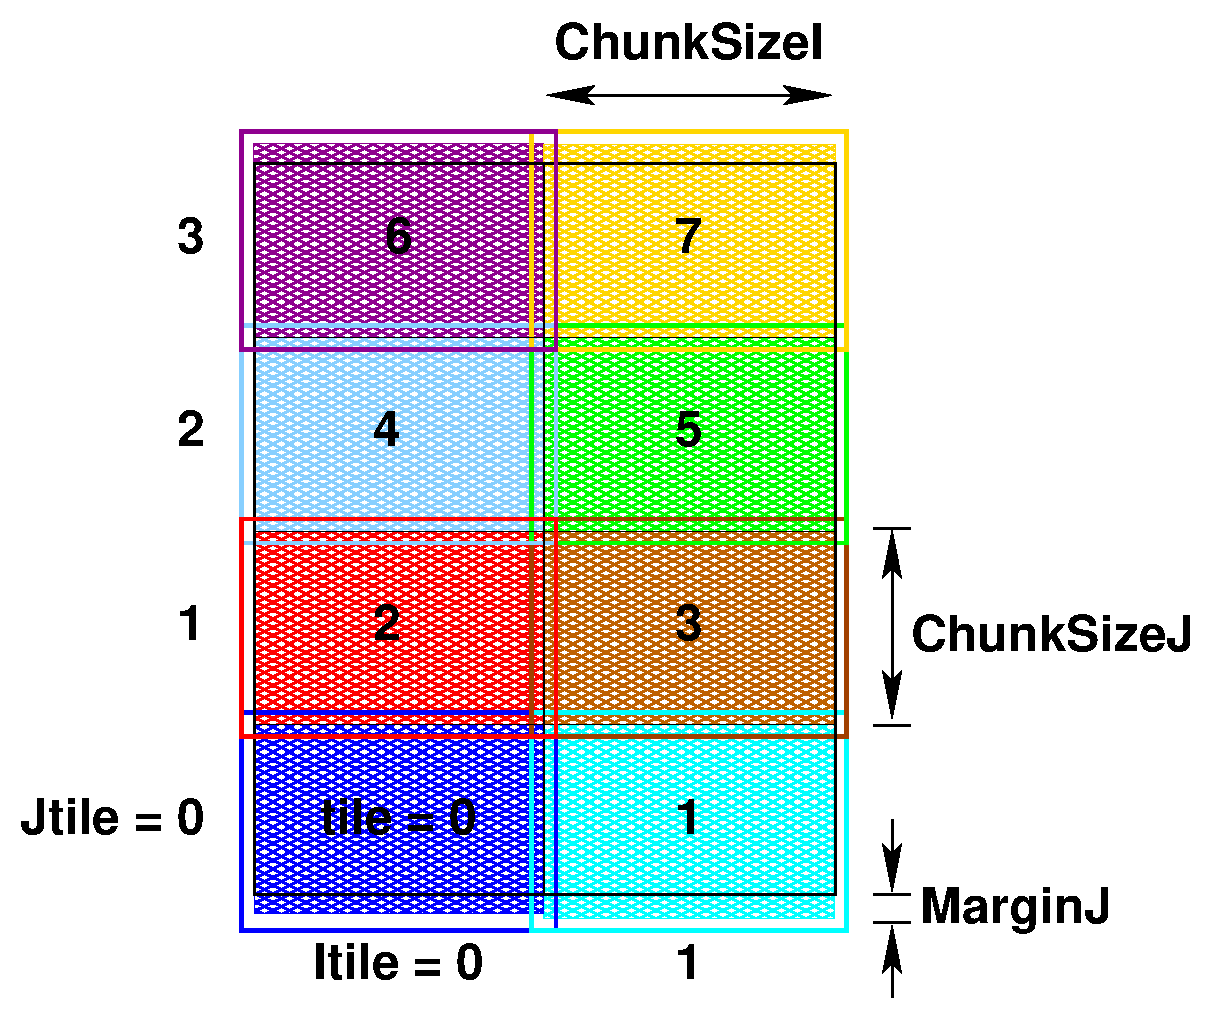
\includegraphics[height=100mm]{pics/tile3}
  \end{picture}
  \caption{A tiled grid with some ROMS tile variables.}
  \label{ftile2}
\end{figure}

In picking a numbering scheme for indices within a tile, there
are two common choices, as shown in Fig.\ \ref{fdecomp1}. Each
tile can be numbered from 1 to \code{ChunksizeI} or it can retain the
numbering it would have in the whole grid. We have chosen this
second option for ease when debugging features such as river
inputs which apply to specific locations on the grid. It is
simple to do using Fortran 90 dynamic memory allocation.

\begin{figure}[t]
\setlength{\unitlength}{10mm}
\begin{picture}(0,7)(0,0)
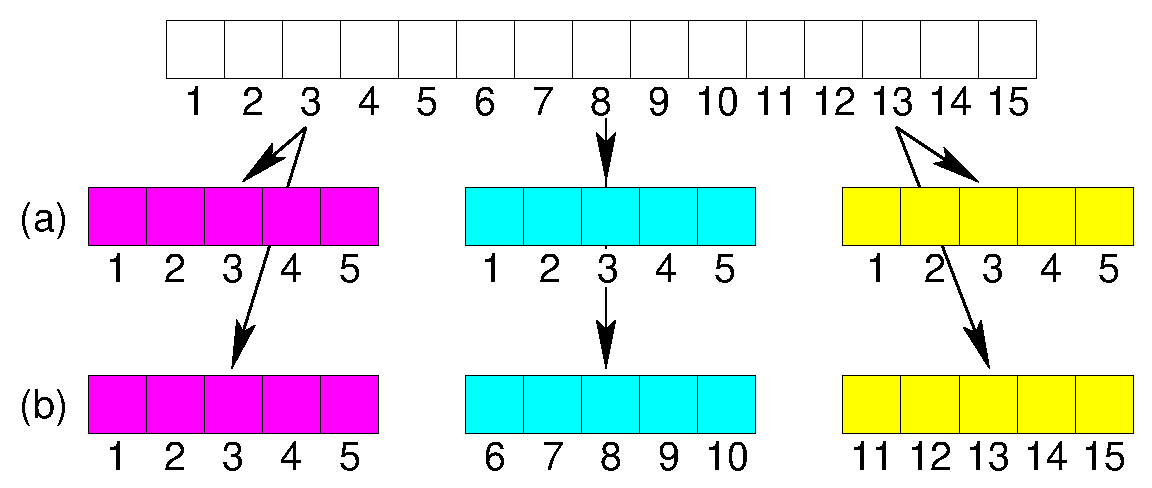
\includegraphics[width=165mm]{pics/numbering}
  \end{picture}
  \caption{A choice of numbering schemes: (a) each tile is numbered
the same, and (b) each tile retains the numbering of the parent
domain.}
  \label{fdecomp1}
\end{figure}

With the tile sizes known, we can assign beginning and ending
indices for each tile. Some of the details depend on whether or
not the domain is periodic in that direction, as shown in Fig.\
\ref{ftile3}.

\begin{figure}[tb]
\setlength{\unitlength}{10mm}
\begin{picture}(0,9)(0,0)
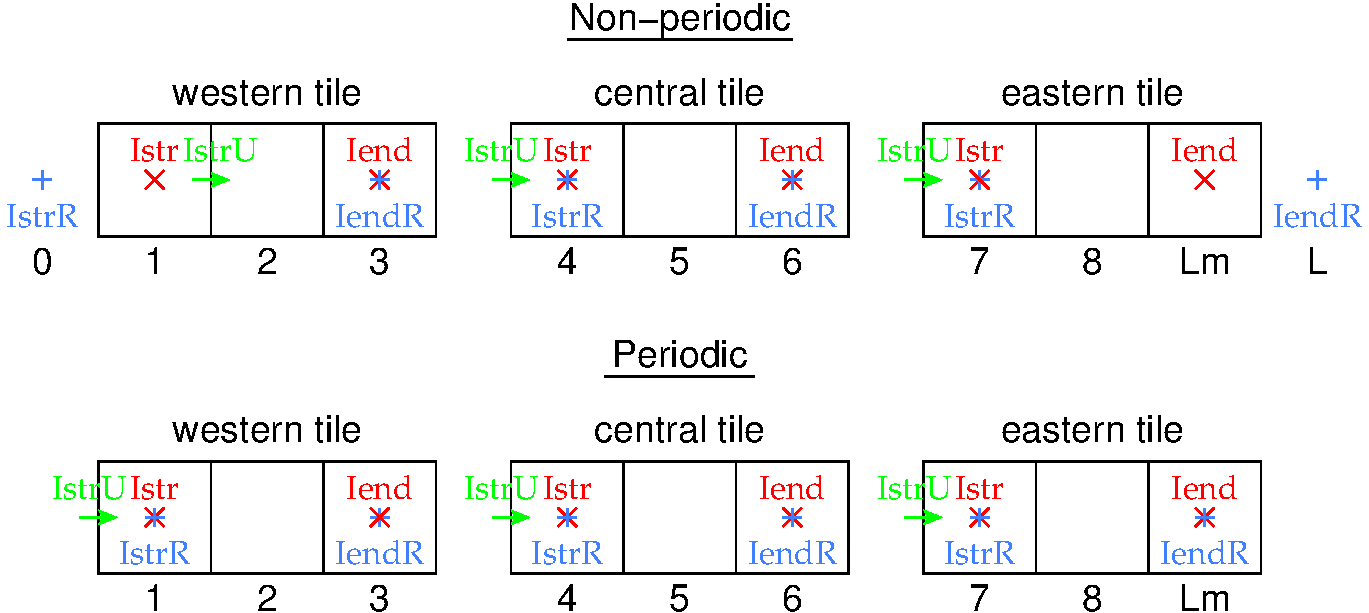
\includegraphics[width=165mm]{pics/Istr}
  \end{picture}
  \caption{Some ROMS variables for tiles, for both a periodic and
  non-periodic case. Shown are the variables in the
  \code{i}-direction, the \code{j}-direction is similar.}
  \label{ftile3}
\end{figure}

\subsubsection{MPI exchange}

For MPI jobs, the ghost points need to be updated between
interior point computations. The routines
\code{mp\_exchange2d}, \code{mp\_exchange3d} and
\code{mp\_exhcnage4d} can be used to update the halo points of
up to four arrays at a time. Each of these routines call
\code{tile\_neighbors} to figure out which tiles are neighboring and
whether or not there really is a neighboring tile on each side. The
\code{mp\_exchangexd} routines then call:
\begin{verbatim}
    mpi_irecv
    mpi_send
    mpi_wait
\end{verbatim}
The exchanges happen first in the east-west direction, then in the
north-south direction, saving the need for diagonal exchanges. A figure
with interior points colored by tile and grey halo points needing an
update is shown in Fig.\ \ref{fex_2d1}(a). The updated halo points are
shown in Fig.\ \ref{fex_2d1}(b).

\begin{figure}[p]
\setlength{\unitlength}{10mm}
\begin{picture}(0,22)(-2.8,0)
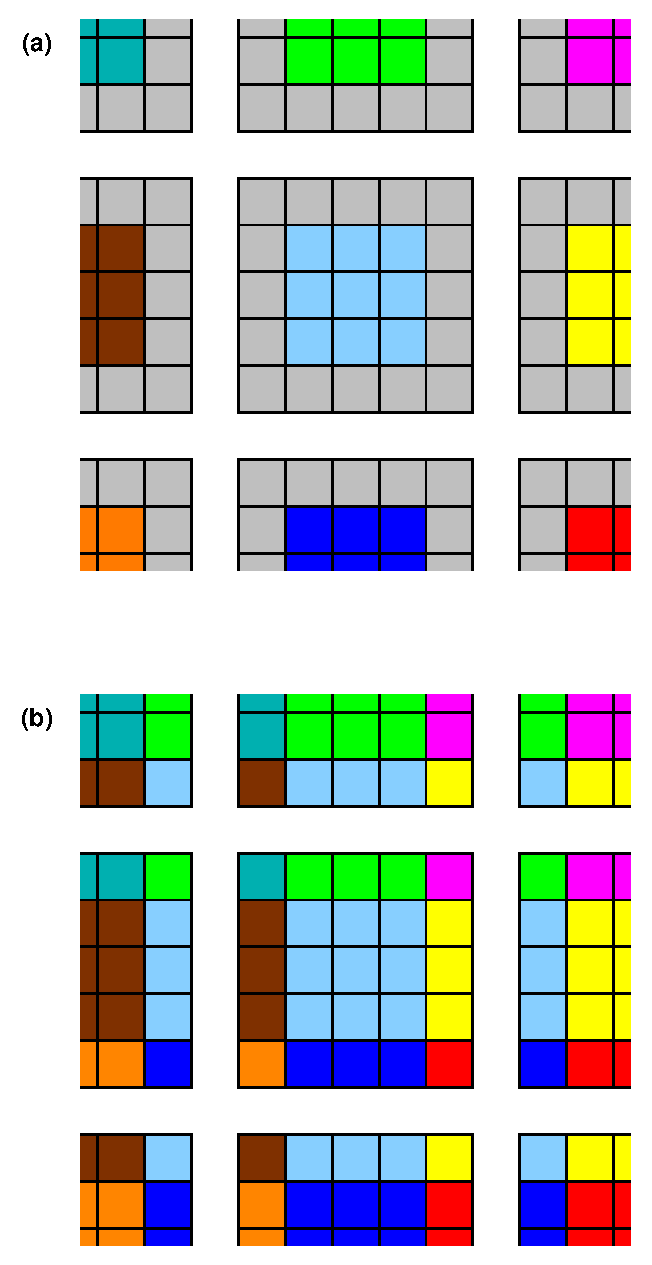
\includegraphics[height=220mm]{pics/ex_2d}
  \end{picture}
  \caption{A tiled grid with out-of-date halo regions shown in
  grey and the interior points color-coded by tile: (a) before an
  exchange and (b) after an exchange.} \label{fex_2d1}
\end{figure}

\subsubsection{Code syntax}

In \code{main3d}, many function calls are surrounded by
OpenMP parallel code such as:
\begin{verbatim}
    !$OMP PARALLEL DO PRIVATE(thread,subs,tile) SHARED(ng,numthreads)
        DO thread=0,numthreads-1
          subs=NtileX(ng)*NtileE(ng)/numthreads
          DO tile=subs*thread,subs*(thread+1)-1,+1
            CALL set_data (ng, TILE)
          END DO
        END DO
    !$OMP END PARALLEL DO 
\end{verbatim}
What isn't obvious from this is that the argument \code{TILE} means
different things depending on if we're using OpenMP or MPI:
\begin{verbatim}
    #ifdef DISTRIBUTE
    # define TILE MyRank
    #else
    # define TILE tile
    #endif
\end{verbatim}
In other words, for MPI, \code{TILE} becomes the process number and
the loop is only executed once.

In looking at a typical routine that's called from \code{main3d},
the routine is usually quite short, calling a \code{\_tile}
version of itself in which the actual work happens:
\begin{verbatim}
    SUBROUTINE set_data (ng, tile)
    # include "tile.h"
      CALL set_data_tile (ng, tile,                        &
     &                    LBi, UBi, LBj, UBj,              &
     &                    IminS, ImaxS, JminS, JmaxS)
      RETURN
      END SUBROUTINE set_data
\end{verbatim}
Here, there are two sets of array lower and upper bounds, those
in the \code{LBi} family and those in the \code{IminS} family. Both
depend on the \code{Istr} family shown in Fig.\ \ref{ftile3}. The
\code{IminS} family is for work arrays that are local to an MPI
process or to an OpenMP thread, also local to a \code{\_tile}
routine. They are initialized:
\begin{verbatim}
      IminS=BOUNDS(ng)%Istr(tile)-3
      ImaxS=BOUNDS(ng)%Iend(tile)+3
      JminS=BOUNDS(ng)%Jstr(tile)-3
      JmaxS=BOUNDS(ng)%Jend(tile)+3
\end{verbatim}
and used:
\begin{verbatim}
      real(r8), dimension(IminS:ImaxS,JminS:JmaxS) ::  work1
      real(r8), dimension(IminS:ImaxS,JminS:JmaxS) ::  work2
\end{verbatim}
The \code{Istr} and \code{LBi} families are dimensioned by the number
of tiles once it is known by \code{inp\_par}:
\begin{verbatim}
        DO ng=1,Ngrids
          Ntiles=NtileI(ng)*NtileJ(ng)-1
          allocate ( BOUNDS(ng) % LBi  (-1:Ntiles) )
                          :
          allocate ( BOUNDS(ng) % Jend (-1:Ntiles) )
        END DO
\end{verbatim}
They are then initialized in calls to the routines in
\code{get\_bounds.F}. If a tile is on the ``western'' edge
(\code{Itile}$=0$), then \code{UBi} is set to \code{LOWER\_BOUND\_I}.
\begin{verbatim}
      Imin=LOWER_BOUND_I
              :
      IF ((Itile.eq.-1).or.(Itile.eq.0)) THEN
        LBi=Imin
      ELSE
        LBi=Istr-Nghost
      END IF
\end{verbatim}
Tracking the origins of \code{LOWER\_BOUND\_I}, we find it in
\code{globaldefs.h}:
\begin{verbatim}
    #ifdef EW_PERIODIC
    #  define LOWER_BOUND_I -GHOST_POINTS
    #else
    #  define LOWER_BOUND_I 0
    #endif
\end{verbatim}

In the case of \code{set\_data}, we are simply passing array indices
for the tiled arrays. To access the tiled arrays from within
\code{set\_data\_tile}, we need to \code{use} the relevant modules
and then refer to the array with its full name:
\begin{verbatim}
      USE mod_forces
            :
      CALL set_2dfld_tile (ng, tile, iNLM, idCfra,             &
     &                     LBi, UBi, LBj, UBj,                 &
     &                     FORCES(ng)%cloudG,                  &
     &                     FORCES(ng)%cloud,                   &
     &                     update)
\end{verbatim}
In other cases, the parent routine would have the \code{use}, then
would pass the relevant array to the \code{\_tile} routine:
\begin{verbatim}
      USE mod_grid
          :
      CALL prsgrd_tile (ng, tile,                              &
          :
     &                  GRID(ng) % Hz,                         &
          :
      SUBROUTINE prsgrd_tile (ng, tile,                        &
          :
     &                        Hz, z_r, z_w,                    &
          :
      real(r8), intent(in) :: Hz(LBi:,LBj:,:)
\end{verbatim}
This allows the \code{\_tile} routine to use \code{Hz} with the same
syntax as the pre-parallel, pre-module code once had.

\subsubsection{Input/output}

In ROMS, the distributed memory I/O is all happening on the master process
(0) unless you specifically ask it to use MPI-I/O, which requires both the
\code{NETCDF4} and \code{PARALLEL\_IO} \code{cpp} flags to be defined.
If you do this, you will be reading and writing \code{HDF5} files and
will need to update your pre- and post-processiong tools accordingly. I
have tentatively tried the parallel I/O and found it to be exceedingly
slow---I've been told since that this is the fault of the \code{NetCDF-4}
layer sitting on top of \code{HDF5}---\code{HDF5} alone should be fast.

In the case of having all the I/O pass through the master process,
we can still read and write classic NetCDF-3 files. Care must be
taken though, in the event of an error. ROMS has been cleaned up so
that the master process will broadcast its return state to the other
processes and they can all die gracefully together when there is a
problem.

An example of a routine which reads from disk is \code{get\_grid},
called from \code{initial}. Each MPI process calls \code{get\_grid}:
\begin{verbatim}
        CALL get_grid (ng, iNLM)
# ifdef DISTRIBUTE
        CALL mp_bcasti (ng, iNLM, exit_flag)
# endif
        if (exit_flag.ne.NoError) RETURN
\end{verbatim}
If any one of the processes has trouble, it will enter into the
\code{exit\_flag} which is then shared by all.

To read in an array variable, all processes in \code{get\_grid} uses
\code{nf\_fread2d} and friends:
\begin{verbatim}
            status=nf_fread2d(ng, model, ncname, ncGRDid(ng),      &
     &                        var_name(it), var_id(it),            &
     &                        0, gtype, Vsize,                     &
     &                        LBi, UBi, LBj, UBj,                  &
     &                        Fscl, Fmin, Fmax,                    &
     &                        GRID(ng) % rmask,                    &
     &                        GRID(ng) % rmask)
            IF (status.ne.nf90_noerr) THEN
              exit_flag=2
              ioerror=status
              EXIT
            END IF
\end{verbatim}
Within \code{nf\_fread2d}, we get to a call to the NetCDF library
from just the master process:
\begin{verbatim}
      IF (InpThread) THEN
        status=nf90_get_var(ncid, ncvarid, wrk, start, total)
            :
      END IF
# ifdef DISTRIBUTE
      CALL mp_bcasti (ng, model, status)
# endif
      IF (status.ne.nf90_noerr) THEN
        exit_flag=2
        ioerror=status
        nf_fread2d=status
        RETURN
      END IF
\end{verbatim}
At this point, the master process has the entire 2-D array stored in
\code{wrk}. This then needs to be divvied out to the various tiles
to their copy of the array in question (stored in the \code{A}
argument to \code{nf\_fread2d}):
\begin{verbatim}
    # ifdef DISTRIBUTE
            CALL mp_scatter2d (ng, model, LBi, UBi, LBj, UBj,         &
         &                     Nghost, MyType, Amin, Amax,            &
    #  if defined READ_WATER && defined MASKING
         &                     NWpts, SCALARS(ng)%IJwater(:,wtype),   &
    #  endif
         &                     Npts, wrk, A)
\end{verbatim}
Something similar happens when writing to output files.
